\documentclass{tufte-handout}

%\geometry{showframe}% for debugging purposes -- displays the margins

\usepackage{amsmath}

% Set up the images/graphics package
\usepackage{graphicx}
\setkeys{Gin}{width=\linewidth,totalheight=\textheight,keepaspectratio}
\graphicspath{{graphics/}}


% The following package makes prettier tables.  We're all about the bling!
\usepackage{booktabs}

% The units package provides nice, non-stacked fractions and better spacing
% for units.
\usepackage{units}

% The fancyvrb package lets us customize the formatting of verbatim
% environments.  We use a slightly smaller font.
\usepackage{fancyvrb}
\fvset{fontsize=\normalsize}

% Small sections of multiple columns
\usepackage{multicol}

% Provides paragraphs of dummy text
\usepackage{lipsum}

% Provides annotated music scores
\usepackage{musicography}

% Fancy header
\usepackage{fancyhdr}

\usepackage{array, boldline, makecell, booktabs}

\newcommand{\bmp}[1]{\begin{minipage}{#1}}
\newcommand{\emp}{\end{minipage}}
\newcommand{\tw}{\textwidth}

% These commands are used to pretty-print LaTeX commands
\newcommand{\doccmd}[1]{\texttt{\textbackslash#1}}% command name -- adds backslash automatically
\newcommand{\docopt}[1]{\ensuremath{\langle}\textrm{\textit{#1}}\ensuremath{\rangle}}% optional command argument
\newcommand{\docarg}[1]{\textrm{\textit{#1}}}% (required) command argument
\newenvironment{docspec}{\begin{quote}\noindent}{\end{quote}}% command specification environment
\newcommand{\docenv}[1]{\textsf{#1}}% environment name
\newcommand{\docpkg}[1]{\texttt{#1}}% package name
\newcommand{\doccls}[1]{\texttt{#1}}% document class name
\newcommand{\docclsopt}[1]{\texttt{#1}}% document class option name


%%% Additions to template by DSL
\usepackage{hyperref} % provides \url{}
% remove separation between list items http://tex.stackexchange.com/a/10689/1783
\usepackage{enumitem}
\setlist{nosep}

%%-- another way
\usepackage{tikzpagenodes}
\newcommand{\mylogo}[1]{%
\tikz[remember picture,overlay] {%
  \node[inner sep=0pt,anchor=east] at ([yshift=+1.0cm, xshift=+7.0cm]current page text area.north east){#1};}
  }

\usepackage{mathrsfs}
\usepackage{tcolorbox}
\tcbuselibrary{theorems}
\usepackage{xcolor}
\usepackage{epsdice}
\usepackage{pgfplots}

\usepackage{graphicx,xspace,color,cancel}
\usepackage{tikz}
\usetikzlibrary{arrows,shapes,backgrounds,through,shadows}
\usetikzlibrary{decorations.pathmorphing}
\usetikzlibrary{calc}

\newcommand{\boxit}[4]
{
\path #2+(-#4,-#4) node(bottomleft){};
\path #3+(#4,#4) node(upperright){};
\draw[rounded corners,black!80] (bottomleft) rectangle (upperright);
%\path (#2-|#3) node(bottomright){};
\path (bottomleft-|upperright) node(bottomright){};
\path (bottomright) node[above left]{#1};
}

\tikzstyle{cont}=[circle, draw,% a shading that is white at the top...
thick,minimum size=6mm,line width=1pt,>=stealth]  % continuous  node
\tikzstyle{dgraph}=[->, line width=1.5pt]
\tikzstyle{ugraph}=[line width=1.5pt]

\tikzstyle{contblk}=[circle, draw=black,top color=black,bottom color=black,% a shading that is white at the top...
thick,minimum size=1mm,line width=1pt,>=stealth]  % continuous  node
\tikzstyle{dgraph}=[->, line width=1.5pt]



\newtcbtheorem[number within=]{mydef}{Definition}%
{colback=DarkOrchid!5,colframe=DarkOrchid!90!black,fonttitle=\bfseries}{th}

\newtcbtheorem[number within=]{mydef2}{Definition$^*$}%
{colback=Rhodamine!5,colframe=Rhodamine!90!black,fonttitle=\bfseries}{th}


\newtcbtheorem[number within=]{mybox}{Box}%
{colback=Aquamarine!5,colframe=Aquamarine!90!black,fonttitle=\bfseries}{th}

\newtcbtheorem[number within=]{mybox2}{Box$^*$}%
{colback=gray!5,colframe=gray!90!black,fonttitle=\bfseries}{th}

\newtcbtheorem[number within=]{mythe}{Theorem}%
{colback=DarkOrchid!5,colframe=DarkOrchid!90!black,fonttitle=\bfseries}{th}



% \bigcupdot
\makeatletter
\def\moverlay{\mathpalette\mov@rlay}
\def\mov@rlay#1#2{\leavevmode\vtop{%
   \baselineskip\z@skip \lineskiplimit-\maxdimen
   \ialign{\hfil$\m@th#1##$\hfil\cr#2\crcr}}}
\newcommand{\charfusion}[3][\mathord]{
    #1{\ifx#1\mathop\vphantom{#2}\fi
        \mathpalette\mov@rlay{#2\cr#3}
      }
    \ifx#1\mathop\expandafter\displaylimits\fi}
\makeatother
\newcommand{\cupdot}{\charfusion[\mathbin]{\cup}{\cdot}}
\newcommand{\bigcupdot}{\charfusion[\mathop]{\bigcup}{\boldsymbol{\cdot}}}

%\rhead{\includegraphics[width=1cm]{fig/T1.png}}
\def\ci{\perp\!\!\!\perp}

\title{Machine Learning }
\author{Salvador Ruiz Correa}
\date{Aprib 26th, 2026}  % if the \date{} command is left out, the current date will be used
\begin{document}

\maketitle% this prints the handout title, author, and date
\mylogo{
\includegraphics[height=15mm]{fig/T2.png}}

\begin{abstract}
\textsc{ The VC (Vapnik-Chervonenkis) dimension} measures the capacity or complexity of a model or hypothesis class in machine learning. It quantifies how well a model can fit a variety of datasets. Specifically, the VC dimension represents the maximum number of data points a model can shatter, meaning it can perfectly classify all possible labelings of those points.
A higher VC dimension indicates that the model is more flexible and capable of learning complex patterns. However, it also suggests a higher risk of overfitting, as the model might capture noise instead of meaningful relationships. Conversely, a low VC dimension suggests limited capacity, which might lead to underfitting.
The VC dimension helps balance the trade-off between model flexibility and generalization. It's a theoretical tool often used in statistical learning theory to evaluate a model's generalization ability to unseen data.
\end{abstract}
\marginnote[-5cm]{
\textsc{Agenda:}
\begin{description}
\item{1} Generalization Error.
\item{2} Effective Number of Hypotheses.
\item{3} The VC Dimension.
\item{4} Approximation-Generalization Tradeoff.
\end{description}
}

\section{Generalization Error}

We have already discussed the value of $E_{{\sf in}}$ does not always generalize to a similar value of $E_{{\sf out}}$.
Generalization is a key issue in learning. One can define the {\em generalization error} as the discrepancy between $E_{{\sf in}}$ an $E_{{\sf out}}$. The Hoeffding Inequality provides a way to characterize the generalization error with a probabilistic bound,

\begin{equation*}
P(|E_{{\sf in}}(g) - E_{{\sf out}}(g) | \ge \epsilon) \leq 2Me^{-2\epsilon^2N},
\end{equation*}
for any $\epsilon > 0$, where $g \in \mathcal H$, $\mathcal H= \{h_1,h_2,\dots, h_M\}$. Pick a tolerance level $\delta$, for example $\delta=0.05$, and assert with probability at least $1-\delta$
\begin{equation*}
E_{{\sf out}}(g)  \leq  E_{{\sf in}}(g)   + \sqrt{\frac{1}{2N}\log\frac{2M}{\delta}}.
\end{equation*}
We call this equation {\em generalization bound} because it bounds $E_{{\sf out}}$ in terms of $E_{{\sf in}}$.

\section{Effective Number of Hypotheses}

The {\em growth function } quantifies the {\em effective} number of hypotheses. The growth function replaces in the generalization bound. It can handle hypothesis spaces of infinite cardinality.


Let $X_1, X_2, \dots, X_N$ be samples from a data generation function. The {\em dichotomies generated} by a hypothesis space $\mathcal H$ on these samples are defined by
\begin{equation*}
\mathcal H(X_1, X_2, \dots, X_N) = \{ \left(h(X_1),h(X_2), \dots, h(X_N) \right)| h \in \mathcal H\}.
\end{equation*}
One can think of the dichotomies $\mathcal H(X_1, X_2, \dots, X_N)$ as a set of hypotheses just like $\mathcal H$, except that the hypotheses are seen through the eyes of $N$ points only. A larger $\mathcal H(X_1, X_2, \dots, X_N)$ means that $\mathcal H$ is more diverse, getting more dichotomies on $X_1, X_2, \dots, X_N$. The growth function is based on the number of dichotomies.

The growth function is defined for a hypothesis set set $\mathcal H$ by
\begin{equation*}
m_{\mathcal H}(N) = \max_{X_1, X_2, \dots, X_N} | \mathcal H(X_1, X_2, \dots, X_N)|
\end{equation*}
where $|\cdot|$ denotes a set's cardinality (number of elements).

In words, $m_{\mathcal H}(N)$ is the maximum number of dichotomies generated on $\mathcal H $ any $N$ points. To compute $m_{\mathcal H}(N)$, we consider all possible choices of $N$ points $X_1, X_2, \dots, X_N$ and pick the ones that give us the most dichotomies. Like $M$, $m_{\mathcal H}(N)$ measures the number of hypotheses in $\mathcal H$, except that a hypothesis is now considered on $N$ points. For any $\mathcal H(X_1, X_2, \dots, X_N)\subseteq \{-1,+1\}^N$ (the set of all possible dichotomies on any N points), the value of  $m_{\mathcal H}(N)$ is at most $|\{-1,+1\}^N|$, hence 
\begin{equation*}
m_{\mathcal H}(N) \leq 2^N.
\end{equation*}
If $\mathcal H$ is capable dichotomies on  of generating all possible $X_1$, $X_2$, $\dots$, $X_N$, then $H(X_1, X_2, \dots, X_N)= \{-1,+1\}^N$, and we say the $\mathcal H$ shatters $X_1$, $X_2$, $\dots$, $X_N$.  This signifies that $\mathcal H$ is as diverse as this sample can be.

If no data set of size $\mathcal H$ can shatter $k$, then it is said to be a {\em breakpoint} for $\mathcal H$.
If the condition of $m_{\mathcal H}(N) = 2^N$ breaks at any point, we can bound $m_{\mathcal H}(N) = 2^N$  for all values of $N$ by a simple polynomial based on this breakpoint.

\begin{mydef}{The VC Dimension }{theoexample}
The Vapnik-Chervonenkis dimension of a hypothesis set $\mathcal H$, denoted by $d_{VC}(\mathcal H)$, is the largest $N$ for which $m_{\mathcal H}(N) = 2^N$. If $m_{\mathcal H}(N)=N $ for all $N$, then $d_{VC}(\mathcal H)=\infty$. 
 \end{mydef}
If  $d_{VC}=\infty$ is the VC dimension of $\mathcal H$, then $k=d_{VC}+1$ is  breakpoint for $m_{\mathcal H}(N) = 2^N$ since $m_{\mathcal H}(N) $ cannot be equal to $2^N$ for any $N>d_{VC}$ by definition. It is easy to see that no smaller breakpoint exists sin ce $\mathcal H$ can shatter $d_{VC}$ points; hence, it can shatter any subset of points.

Note that if $m_{\mathcal H}(N)\leq 2^k$ for some value $k$, then 
\begin{equation*}
m_{\mathcal H}(N) \leq \sum_{i=0}^{k} \binom{N}{i}
\end{equation*}
for all $N$. The RHS is polynomial in $N$ of degree $k-1$.  Since $k  = d_{VC} +1 $ is a breakpoint for $m_{\mathcal H}(N)$,
\begin{equation*}
m_{\mathcal H}(N) \leq \sum_{i=0}^{d_{VC}} \binom{N}{k}
\end{equation*}
From these results, we can show that 
\begin{equation*}
m_{\mathcal H}(N) \leq N^{d_{VC}} +1.
\end{equation*}

\section{The VC Generalization Bound }

For any tolerance $\delta >0$,
\begin{equation*}
E_{{\sf out}} \leq E_{{\sf in}} +\sqrt{\frac{8}{N} \log \frac{4m_{\mathcal H}(2N)}{\delta}}
\end{equation*}
with probability $\geq 1 - \delta $

Another valid bound can be obtained using the $d_{VC}$ polynomial bound. 
\begin{equation*}
E_{{\sf out}} \leq E_{{\sf in}} +\sqrt{\frac{8}{N} \log \frac{4((2N)^{d_{VC}} + 1)}{\delta}}
\end{equation*}

We can write 
\begin{equation*}
E_{{\sf out}} \leq E_{{\sf in}} + \Omega(N,\mathcal H,S)
\end{equation*}
where
\begin{equation*}
\Omega(N,\mathcal H,S) = \sqrt{\frac{8}{N} \log \frac{4m_{\mathcal H}(2N)}{\delta}},
\end{equation*}
or 
\begin{equation*}
\Omega(N,\mathcal H,S) = \sqrt{\frac{8}{N} \log \frac{4((2N)^{d_{VC}} + 1)}{\delta}}.
\end{equation*}

\begin{figure}
\includegraphics[width=9cm]{fig/lcurve0.png}
\caption{Learning curves. From Learning from Data.}
\label{fig:ubc}
\end{figure}

\begin{figure}
\includegraphics[width=11cm]{fig/lcurves.png}
\caption{Learning curves. From Learning from Data.}
\label{fig:ubc}
\end{figure}



\section{Approximation-Generalization Tradeoff}

There is another way to look at the approximation-generalization tradeoff
that is particularly suited for squared error measures rather than the binary error used in the VC analysis. 

The bias-variance decomposition of the out-of-sample error is based on squared error measures. 

As an example, consider the case of a polynomial regression. Let $\mathcal D = (\{x_1,t_1\},\{x_2,t_2\}, \dots \{x_N,t_N\})$  an i.i.d. sample (training set)  where
\begin{align*}
x \sim p(x),
\end{align*}
and 
\begin{align*}
t= f(x)  = \sin(2\pi x) + \epsilon(x),
\end{align*}
with
\begin{align*}
  \epsilon(x) \sim \mathcal N (x\mid 0,\sigma^2) ,
\end{align*}
Therefore:
\begin{align*}
t \mid x \sim \mathcal N (x \mid \sin(2\pi x),\sigma^2).
\end{align*}
The graphical model associated with the sample is:
\begin{center}
\scalebox{.9}{
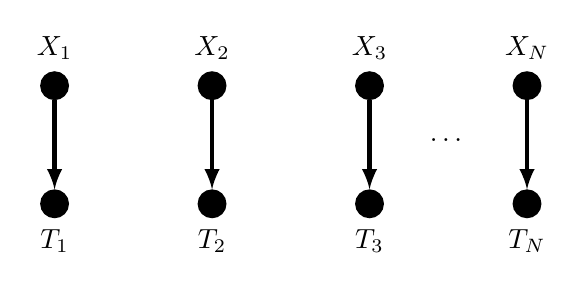
\begin{tikzpicture}[dgraph]
\node[contblk,label=above:{$X_1$}] (x1) at (0,0) {};
\node[contblk, label=below:{$T_1$}] (t1) at (0, -1.5) {};
\node[contblk, label=above:{$X_2$}] (x2) at (2, 0) {};
\node[contblk, label=below:{$T_2$}] (t2) at (2,-1.5) {};
\node[contblk, label=above:{$X_3$}] (x3) at (4, 0) {};
\node[contblk, label=below:{$T_3$}] (t3) at (4, -1.5) {};
\node[contblk, label=above:{$X_N$}] (xN) at (6, 0) {};
\node[contblk, label=below:{$T_N$}] (tN) at (6, -1.5) {};
\node[label={$\dots$}] (A) at (5, -1) {};
\draw [-{latex[slant=0]}]  (x1) -- (t1);
\draw [-{latex[slant=0]}] (x2) -- (t2);
\draw [-{latex[slant=0]}] (x3) -- (t3);
\draw [-{latex[slant=0]}]  (xN) -- (tN);
\end{tikzpicture}}
\end{center}

The conditional  likelihood of the model is
\begin{align*}
p(t_1,t_2,\dots,t_N\mid  x_1,x_2,\dots,x_N) = \prod_{n=1}^N \mathcal N (\sin(2\pi x_n)\mid 0,\sigma^2),
\end{align*}
and the joint distribution of the sample  is:
\begin{align*}
p(\mathcal D) = p(t_1,t_2,\dots,t_N, x_1,x_2,\dots,x_N) = \prod_{n=1}^N \mathcal N (\sin(2\pi x_n)\mid 0,\sigma^2)p(x_n),
\end{align*}
and the joint distribution over $M$ training sets is
\begin{align*}
p(\mathcal D_M) = \prod_{m=1}^Mp(t_{m1},t_{m2},\dots,t_{mN}, x_{m1},x_{m2},\dots,x_{mN}) = \prod_{m=1}^M\prod_{n=1}^N \mathcal N (\sin(2\pi x_{mn})\mid 0, \sigma^2) p(x_{mn}).
\end{align*}

Assume we conducted an MLE estimation of the polynomial coefficients based on the data sample to get a specific solution $g(x)$ from the hypotheses space $ g\in \mathcal H$.  Clearly,
\begin{align*}
t = g(x) = g(x; \underbrace{t_{1},t_{2},\dots,t_{N}, x_{1},x_{2},\dots,x_{N}}_{\sim p(\mathcal D)}).
\end{align*}

By definition, the out-of-sample error is:
\begin{align*}
\mathrm E_{\mathsf{ out}}(g^{\mathcal D}) &= \mathrm E_x [ (g^{\mathcal D}(x) - f(x))^2 ] \\ &= 
\mathrm E_x  [g^{\mathcal D}(x)^2 ] - 2 \mathrm E_x  [g^{\mathcal D}(x) f(x)] + 
E_x  [ f(x)]
\end{align*}
and the expected value of $\mathrm E_{\mathsf{ out}}(g^{\mathcal D})$ with respect to $p(\mathcal D)$ is
\begin{align*}
\mathrm E_{\mathcal D} \left[ \mathrm E_{\sf out} (g^{\mathcal D}) \right]&=  \mathrm E_{\mathcal D}\left[\mathrm E_{ x}\left[ (g^{\mathcal D}(x) -f(x))^2 \right] \right]\\
&= \mathrm E_{x}\left[\mathrm E_{\mathcal D}\left[ (g^{\mathcal D}(x) -f(x))^2 \right] \right]\\
\end{align*}
since the expected value is a linear operator, and where:
\begin{align*}
E_{\mathcal D}\left[ (g^{\mathcal D}( x) -f(\mathbf x))^2 \right] = \int (g^{\mathcal D}(x) -f( x))^2 p(\mathcal D) d\mathcal D.
\end{align*}
Notice that taking the expectation concerning all data sets eliminates dependence on any particular data set.


\begin{figure}
\includegraphics[width=12cm]{fig/lcurves2.png}
\caption{Learning curves. From Learning from Data.}
\label{fig:ubc}
\end{figure}




			
In general for a deterministc function  $f(\mathbf x)$, the bias variance decomposition is:
\begin{align*}
\mathrm E_{\mathcal D} \left[ \mathrm E_{\sf out} (g^{\mathcal D}) \right]&=  \mathrm E_{\mathcal D}\left[\mathrm E_{\mathbf x}\left[ (g^{\mathcal D}(\mathbf x) -f(\mathbf x))^2 \right] \right]\\
&= \mathrm E_{\mathbf x}\left[\mathrm E_{\mathcal D}\left[ (g^{\mathcal D}(\mathbf x) -f(\mathbf x))^2 \right] \right]\\
&= \mathrm E_{\mathbf x}\left[\mathrm E_{\mathcal D}\left[ g^{\mathcal D}(\mathbf x)^2\right] -  2 \underbrace{E_{\mathcal D}\left[ g^{\mathcal D}(\mathbf x)\right]}_{\mathsf{average \, function\,over\, \mathcal D}}f(\mathbf x)  + f(\mathbf x)^2  \right]\\
&= \mathrm E_{\mathbf x}\left[\mathrm E_{\mathcal D}\left[ g^{\mathcal D}(\mathbf x)^2\right] -  2 \bar{g}(\mathbf x)f(\mathbf x)  + f(\mathbf x)^2  \right]\\
&= \mathrm E_{\mathbf x}\left[\mathrm E_{\mathcal D}\left[ g^{\mathcal D}(\mathbf x)^2\right] - \bar{g}(\mathbf x)^2 + \bar{g}(\mathbf x)^2 - 2 \bar{g}(\mathbf x)f(\mathbf x)  + f(\mathbf x)^2  \right]\\
&= \mathrm E_{\mathbf x}\left[\mathrm E_{\mathcal D}\left[ g^{\mathcal D}(\mathbf x)^2\right] - \bar{g}(\mathbf x)^2 +   (\bar{g}(\mathbf x) - f(\mathbf x))^2  \right]\\
&= \mathrm E_{\mathbf x}\left[\mathrm E_{\mathcal D}\left[ (g^{\mathcal D}(\mathbf x)  - \bar{g}(\mathbf x))^2\right] +   (\bar{g}(\mathbf x) - f(\mathbf x))^2  \right]\\
&= \mathrm E_{\mathbf x}\left[ \underbrace{\mathrm E_{\mathcal D}\left[ (g^{\mathcal D}(\mathbf x)  - \bar{g}(\mathbf x))^2\right]}_{\mathsf{variance(x)}}\right]  +  \mathrm E_{\mathbf x} \left[ \underbrace{ (\bar{g}(\mathbf x) - f(\mathbf x))^2}_{\mathsf{bias(x)}} \right] \\\
&=  \mathrm E_{\mathbf x}\left[ \mathsf{variance(\mathbf x)}  \right] + \mathrm E_{\mathbf x}\left[ \mathsf{bias(\mathbf x)}  \right]\\
&= \mathsf{bias + variance}.
\end{align*}

When $M$ data sets are considered for learning, each data set will lead to a particular solution $g_m(x)$ and, therefore:
\begin{align*}
\bar{g}(\mathbf x) \approx \frac{1}{M}\sum_{m=1}^M g_m(\mathbf x).
\end{align*}

%{Explanation of Terms:}
%\begin{itemize}
 %   \item  {Bias} (\( \text{Bias}^2 \)): Error due to incorrect model assumptions or underfitting. For example, a linear model approximating a nonlinear \( f(x) \).
%    \item  {Variance}: Error due to the model's sensitivity to small fluctuations in the training data (overfitting).
%    \item  {Irreducible Error} (\( \sigma^2 \)): Error inherent in the noise \( \epsilon \), which no model can reduce.
%\end{itemize}

This decomposition highlights the trade-off between bias and variance, which is crucial in model selection and regularization.

\begin{mybox}{Example $t(x) = f(x) + \epsilon(x) $}{theoexample}

The {bias-variance decomposition} provides a framework to analyze the error of a learning algorithm by separating it into three components: {bias}, {variance}, and {irreducible error}. 

Let us derive it for the function \( t(x) = f(x) + \epsilon(x) \), where \( f(x) \) is the deterministic (true) function; and \( \epsilon = \epsilon(x)\) is Gaussian noise with zero mean and variance \( \sigma^2 \). Now suppose we use a model \(g(x) \) to estimate \( f(x) \). The prediction error for a given \( x \) is measured as the  {mean squared error} (MSE) of \(g(x) \) with respect to the true target \( t(x) \):
\begin{align*}
\text{MSE} &= \mathrm{E_x} \big[(t -g(x))^2\big] \\
&= \mathrm{E_x} \big[(f(x) + \epsilon -g(x))^2\big].
\end{align*}
Taking the expectation wrt  $p(\mathcal D)$ and expanding the square:
\[
\mathrm E_{\mathcal D} \big[ \text{MSE} \big]= \mathrm E_{\mathcal D} \big[ \mathrm{E_x} \big[(f(x) -g(x))^2 + 2\epsilon(f(x) -g(x)) + \epsilon^2\big]\big].
\]

Since  \( \epsilon \) is independent of \(g(x) \), and the mean is zero, the cross-term vanishes:
$
\mathrm{E_x}[\epsilon(f(x) -g(x))] = 0.
$

This simplifies to:
\[
\mathrm E_{\mathcal D} \big[  \text{MSE}\big] = \mathrm E_{\mathcal D} \big[  \mathrm{E_x} \big[(f(x) -g(x))^2\big] + \mathrm{E_x}[\epsilon^2] \big].
\]

Recalling that \( \mathrm{E_x}[\epsilon^2] = \sigma^2 \), we have:
\begin{align*}
\mathrm E_{\mathcal D} \big[\text{MSE} \big]&=  \mathrm E_{\mathcal D} \big[\mathrm{E_x} \big[(f(x) -g(x))^2\big] + \sigma^2 \big]\\
&=  \mathrm E_{\mathcal D} \big[\mathrm{E_x} \big[(f(x) -g(x))^2\big] \big] + \sigma^2\\
&=  \mathrm E_{x} \big[\mathrm{E_{\mathcal D}} \big[(f(x) -g(x))^2\big] \big] + \sigma^2.
\end{align*}
The term \( \mathrm{E_{\mathcal D}} \big[(f(x) -g(x))^2\big] \) can be further decomposed. Let \( \bar{g}(x) = \mathrm{E_{\mathcal D}}[g(x)] \) denote the expected prediction of the model across data sets. Then:
\[
\mathrm{E_{\mathcal D}} \big[(f(x) -g(x))^2\big] = \big(f(x) - \bar{g}(x)\big)^2 + \mathrm{E_{\mathcal D}} \big[(g(x) - \bar{g}(x))^2\big].
\]

Here:
\begin{itemize}
    \item \( \big(f(x) - \bar{g}(x)\big)^2 \) is the {squared bias}: it measures how far the average prediction of the model is from the true function \( f(x) \), for a given $x$.
    \item \( \mathrm{E_{\mathcal D}} \big[(g(x) - \bar{g}(x))^2\big] \) is the  {variance}: it measures the variability of the model's predictions around its mean prediction, for a given $x$.
\end{itemize}
Finally:
\begin{align*}
\mathrm E_{\mathcal D}  \big[ \text{MSE} \big]&=  \mathrm{E_x} \big[ \big(f(x) - \bar{g}(x)\big)^2 \big]+  \mathrm{E_x} \big[ \mathrm{E_{\mathcal D}} \big[(g(x) - \bar{g}(x))^2\big] \big]+ \sigma^2\\ &= \mathsf{bias + variance} + \sigma^2.
\end{align*}


\end{mybox}


\section*{Expectation of a Random Variable}

The \textbf{expectation} (or \textbf{expected value}) of a random variable is a fundamental concept in probability theory that provides a measure of the center of the distribution of the random variable. It is often denoted by \( \mathrm{E}[X] \) for a random variable \( X \).

\subsection*{Expectation for a Discrete Random Variable}

For a \textbf{discrete random variable} \( X \) with possible values \( x_1, x_2, \dots \) and corresponding probabilities \( p_1, p_2, \dots \), the expectation is calculated as:

\[
\mathrm{E}[X] = \sum_{i} x_i \cdot p_i
\]

where \( p_i = P(X = x_i) \).

\subsection*{Expectation for a Continuous Random Variable}

For a \textbf{continuous random variable} \( X \) with probability density function (PDF) \( f(x) \), the expectation is calculated as:

\[
\mathrm{E}[X] = \int_{-\infty}^{\infty} x \cdot f(x) \, dx
\]

\section*{Expectation of Several Random Variables}

When dealing with multiple random variables, the expectation can be extended to functions of these variables.

\subsection*{Expectation of a Function of Random Variables}

Let \( X \) and \( Y \) be random variables, and let \( g(X, Y) \) be a function of \( X \) and \( Y \). The expectation of \( g(X, Y) \) is given by:

\[
\mathrm{E}[g(X, Y)] = \begin{cases}
\sum_{x} \sum_{y} g(x, y) \cdot P(X = x, Y = y) & \text{(discrete case)} \\
\int_{-\infty}^{\infty} \int_{-\infty}^{\infty} g(x, y) \cdot f_{X,Y}(x, y) \, dx \, dy & \text{(continuous case)}
\end{cases}
\]
where \( f_{X,Y}(x, y) \) is the joint probability density function of \( X \) and \( Y \).

\subsection*{Linearity of Expectation}

One of the most important properties of expectation is its linearity. For any random variables \( X \) and \( Y \), and constants \( a \) and \( b \), the following holds:

\[
\mathrm{E}[aX + bY] = a\mathrm{E}[X] + b\mathrm{E}[Y]
\]

This property holds regardless of whether \( X \) and \( Y \) are independent or not.

\subsection*{Expectation of Independent Random Variables}

If \( X \) and \( Y \) are {independent} random variables, then the expectation of their product is the product of their expectations:

\[
\mathrm{E}[XY] = \mathrm{E}[X] \cdot \mathrm{E}[Y]
\]

This special case arises from the independence of \( X \) and \( Y \).


\begin{itemize}

\item Expectation of a Single Random Variable: For a discrete random variable, the expectation is the sum of each possible value multiplied by its probability. For a continuous random variable, the expectation is the integral of the value multiplied by its probability density function.

\item Expectation of Several Random Variables: The expectation can be extended to functions of multiple random variables, either through summation (for discrete variables) or integration (for continuous variables). The linearity of expectation allows us to compute the expectation of linear combinations of random variables efficiently. For independent random variables, the expectation of their product is the product of their expectations.

\end{itemize}



\section*{Properties of Mathematical Expectation}

Let \( X \) and \( Y \) be random variables, and let \( a \) and \( b \) be constants. The following are the key properties of mathematical expectation:

\subsection*{1. Linearity of Expectation}
The expectation operator is linear. For any constants \( a \) and \( b \),
\[
\mathrm{E}[aX + bY] = a\mathrm{E}[X] + b\mathrm{E}[Y].
\]
This property holds regardless of whether \( X \) and \( Y \) are independent.

\subsection*{2. Expectation of a Constant}
The expectation of a constant \( c \) is the constant itself:
\[
\mathrm{E}[c] = c.
\]

\subsection*{3. Expectation of a Function of a Random Variable}
For any function \( g(X) \) of a random variable \( X \),
\[
\mathrm{E}[g(X)] = \begin{cases}
\sum_{x} g(x) \cdot P(X = x) & \text{(discrete case)} \\
\int_{-\infty}^{\infty} g(x) \cdot f_X(x) \, dx & \text{(continuous case)}
\end{cases}
\]
where \( f_X(x) \) is the probability density function of \( X \).

\subsection*{4. Expectation of Independent Random Variables}
If \( X \) and \( Y \) are independent random variables, then
\[
\mathrm{E}[XY] = \mathrm{E}[X] \cdot \mathrm{E}[Y].
\]
This property does not hold if \( X \) and \( Y \) are dependent.

\subsection*{5. Monotonicity of Expectation}
If \( X \leq Y \) almost surely (i.e., with probability 1), then
\[
\mathrm{E}[X] \leq \mathrm{E}[Y].
\]

\subsection*{6. Expectation of a Product of Random Variables}
For any two random variables \( X \) and \( Y \),
\[
\mathrm{E}[XY] = \mathrm{E}[X]\mathrm{E}[Y] + \text{Cov}(X, Y),
\]
where \( \text{Cov}(X, Y) = \mathrm{E}[(X - \mathrm{E}[X])(Y - \mathrm{E}[Y])] \) is the covariance of \( X \) and \( Y \).

\subsection*{7. Expectation of a Sum of Random Variables}
For any two random variables \( X \) and \( Y \),
\[
\mathrm{E}[X + Y] = \mathrm{E}[X] + \mathrm{E}[Y].
\]
This property extends to any finite number of random variables.

\subsection*{8. Expectation of a Conditional Expectation}
The law of iterated expectation states that
\[
\mathrm{E}[X] = \mathrm{E}[\mathrm{E}[X \mid Y]],
\]
where \( \mathrm{E}[X \mid Y] \) is the conditional expectation of \( X \) given \( Y \).

\subsection*{9. Non-Negativity of Expectation}
If \( X \geq 0 \) almost surely, then
\[
\mathrm{E}[X] \geq 0.
\]

\subsection*{10. Jensen's Inequality}
If \( \phi \) is a convex function, then
\[
\phi(\mathrm{E}[X]) \leq \mathrm{E}[\phi(X)].
\]
If \( \phi \) is concave, the inequality is reversed:
\[
\phi(\mathrm{E}[X]) \geq \mathrm{E}[\phi(X)].
\]




\subsection{Excercise}

Assume that $X$ and $Y$ are independent. Show that
\begin{align*}
\mathrm{E}[g(X,Y)] &= \mathrm{E_Y}[ \mathrm{E_X}[ g(X,Y)]]\\
&=\mathrm{E_X}[ \mathrm{E_Y}[ g(X,Y)]].
\end{align*}

\end{document}
\section{Learning from Data}

\noindent \textsc{ Learning from data} refers to deriving insights, models, or solutions based on data, especially in cases where a precise analytical or theoretical solution is either unavailable or too complex to construct. Instead of relying on pre-existing equations or models, we leverage collected data to create an empirical solution that captures patterns and behaviors inherent in the data itself. 

This approach is remarkably versatile, covering many applications across scientific disciplines, engineering, and beyond.  In science, learning from data enables researchers to identify trends and make predictions in complex systems, from climate modeling to genetic research, where data can reveal insights that are difficult to deduce theoretically. 


Engineering underpins robotics, autonomous systems, and control engineering advancements, allowing machines to improve performance through data-driven learning algorithms. This method also has broad applications in medicine, finance, and social sciences, where large datasets can reveal associations and predictive patterns that aid in decision-making, diagnosis, and resource allocation.

Overall, learning from data is a foundational approach to solving real-world problems. Its adaptability to the availability and richness of data reassures us of its applicability, making it one of the most widely used techniques in modern problem-solving across diverse fields.





\section{The Learning Problem}


\begin{marginfigure}
\includegraphics[width=3cm]{fig/ubc.png}
\caption{Is there evidence of breast cancer in this ultrasound image?}
\label{fig:ubc}
\end{marginfigure}

You'll likely get the correct answer if you show a picture to a three-year-old and ask if it includes a tree. But if you ask a thirty-year-old to define a tree, the response might be vague or inconclusive. We don’t learn what a tree is by studying its formal definition; we learn by seeing trees. In other words, we learn from data. Similarly, a radiology student requires extensive training hours to identify abnormalities in imaging studies. Viewing images is essential to a radiologist's education (Figures \ref{fig:ubc} and \ref{fig:bcts}).  

\begin{figure*}
\includegraphics[width=9cm]{fig/bcts.png}
\caption{Examples of abnormal breasts ultrasounds.}
\label{fig:bcts}
\end{figure*}

The core idea of learning from data involves using a set of observations to reveal an underlying process. This broad concept does not easily fit within a single framework. Consequently, various learning paradigms have emerged to address different scenarios and assumptions. In this section, we introduce several of these paradigms. The learning approach we have covered is supervised learning, the most studied and commonly applied type. However, it is not the only approach. Some variations of supervised learning are straightforward enough to fit within the same framework. In contrast, others are more complex and introduce new concepts and techniques that become distinct areas of study. The most significant variations stem from the nature of the dataset.

\newthought{Supervised learning} is a machine learning approach where a model learns from labeled data to make predictions or classify new data. In this paradigm, the dataset includes input-output pairs, where each input is paired with a correct output or label. The model uses these pairs to learn the relationship between inputs and outputs, minimizing errors between its predictions and the actual labels. Common examples include image classification, spam detection, and regression tasks.

\begin{figure*}
\includegraphics[width=16cm]{fig/classifiers.png}
\caption{Classifiers.}
\label{fig:bcts}
\end{figure*}


\newthought{Unsupervised learning}, on the other hand, deals with unlabeled data. The goal is to find patterns or structures in the data without guidance from pre-labeled outputs. Instead of predicting specific labels, the model identifies inherent patterns, clusters, or associations within the dataset. This approach is beneficial for tasks such as clustering, anomaly detection, and market segmentation, where the goal is to discover natural groupings or patterns in data.

\newthought{Reinforcement learning} is a different paradigm where an agent learns by interacting with an environment and receiving feedback in the form of rewards or penalties based on their actions. The agent aims to maximize cumulative rewards over time by learning an optimal policy or strategy. Unlike supervised learning, which requires labeled data, reinforcement learning relies on trial and error, adjusting actions based on the feedback received. It is commonly applied in robotics, game playing, and real-time decision-making tasks where the environment may change and actions directly influence outcomes.

\newthought{Deep learning} is a subset of machine learning tools that uses artificial neural networks with multiple layers, or deep architectures, to learn complex patterns in large datasets. Inspired by the human brain, deep learning models consist of interconnected layers of nodes, or neurons, each layer transforming the data to capture increasingly abstract features. This approach has proven especially powerful in tasks like image and speech recognition, natural language processing, and autonomous driving, where high-level feature extraction is critical.

\begin{figure*}

\includegraphics[width=12cm]{fig/ml.png}
\caption{Machine learning algorithms.}
\label{fig:ml}
\end{figure*}


\section{Capacity, Overfitting and Underfitting}

\noindent \textsc{ Capacity, overfitting, and underfitting} are critical concepts in machine learning that impact the performance and generalization of models. Finding the right balance in model capacity is crucial for achieving optimal performance in machine learning. Balancing capacity helps prevent underfitting, where the model is too simple, and overfitting, where the model is too complex and memorizes noise. Techniques like regularization, cross-validation, and proper model selection contribute to achieving this balance and building models that generalize well to new, unseen data.

Recall that the central challenge in machine learning is that we must perform well on new, previously unseen inputs—not just those on which
 our model was trained. The ability to perform well on previously unobserved inputs is called \textit{generalization}.  The generalization error is defined as the expected value of the error on a new input. Here, the expectation is taken across different possible inputs, drawn from the \textit{distribution of inputs} we expect the system to encounter in practice. 
 \vspace{-0\baselineskip}\footnotetext{Source:Goodfellow I. J.,  Bengio Y.,  and  Courville A. (2016). Deep Learning, MIT Press.}
\vspace{0\baselineskip}
 
Also, recall that a probability distribution over datasets generates the train and test data called the \textit{data-generating process}. We typically make a set of assumptions known collectively as the \textit{i.i.d. assumptions}. These assumptions are that the examples in each dataset are independent and that the train set and test set are identically distributed, drawn from the same probability distribution. This assumption allows us to describe the data-generating process with a probability distribution over a single example. The same distribution is then used to generate every training and testing example. We call that shared underlying distribution the data-generating distribution. This probabilistic framework and the i.i.d. assumptions allow us to study the relationship between training and test errors mathematically.
%\begin{marginfigure}
%
\includegraphics{fig/signal.png}
%\caption{Green dots represent data samples computed as $t=\sin(2\pi x) + \epsilon(x)$, for a set of $x$ input data where $\epsilon$ represents random noise.  The signal $\sin(2\pi x)$ is represented as a continuous signal.   }
%\end{marginfigure}

\begin{mybox}{Training, Testing and Validation Errors}{}
\begin{itemize}
 \item The {\em out-of-sample error (testing error)}  $E_{{\sf out}}$ measures how well our training data has {\em generalized}
to data that we have not seen before. $E_{{\sf out}}$  is based on the performance over the entire feature (input space).
Intuitively, if we want to estimate the value of $E_{{\sf out}}$ using a sample of data points, these points must be new test points that have not 
been used for training. 
\item The {\em in-sample error (training error)} $E_{{\sf in}}$, by contrast, is based on data points that have been used for training. It expressly 
measures training performance. 
\item The {\em generalization error} is defined here as the discrepancy between $E_{{\sf in}}$ and $E_{{\sf out}}$. A small generalization error
suggests that the learning algorithm can generalize over new data.
\item The {\em validation set } is similar to the test set. However, it is not directly used for training. It is used to make certain decisions during the 
learning process. The {\em validation error} is denoted as $E_{{\sf val}}$.
\item The validation set is created as follows. The data set of size $N$  is partitioned into the training set of size $(N-K)$ and a validation set of size $K$.
\item Notice that the minute a set affects the learning process in any way is no longer a test set. However, we will show that the way the validation set is used
in the learning process is so benign that the estimation of $E_{{\sf out}}$ remains almost intact.
\end{itemize} 
\end{mybox}



\section{Classification Example}

Consider a synthetically generated data set representing measurements from a pipeline containing oil, water, and gas (Bishop and James, 1993). These three materials can be present in one of three different geometrical configurations known as ‘homogenous’ (red),  ‘annular,’  (green), and ‘laminar’ (blue), and the fractions of the three materials can also vary. Each data point comprises a 12-dimensional input vector consisting of measurements taken with gamma-ray densitometers that measure the attenuation of gamma rays passing along narrow beams through the pipe. Figure 5 shows 100 points from this data set on a plot showing two measurements $x_6$ and $x_7$ (the remaining ten input values are ignored for this illustration). Each data point is labeled according to which of the three geometrical classes it belongs to, and our goal is to use this data as a training set to classify a new observation $(x_6, x_7 )$, such as the one denoted by the cross in Figure 5. Numerous red points surround the cross so it may belong to the red class. However, plenty of green points are nearby, so it could instead belong to the green class. It seems unlikely that it belongs to the blue class. The intuition here is that the identity of the cross should be determined more strongly by nearby points from the training set and less strongly by more distant points. This intuition is reasonable and will be discussed more fully later on. How can we turn this intuition into a learning algorithm?

\begin{figure}[t]
\includegraphics{fig/oil1.png}
\caption{Oil types dataset.
}
\end{figure}

\newthought{In supervised learning} our goal is to determine a prediction function $h: \mathcal X\rightarrow \mathcal Y$ :  from an input space $\mathcal X$ to an output space $Y$ such that, given $x \in \mathcal X$ , the value $h(x)$ offers an accurate prediction about the true output $y$. Our goal is to choose a prediction function that avoids rote memorization and instead generalizes the concepts that can be learned from a given set of examples. To do this, one should choose the prediction function h by attempting to minimize a risk measure over an adequately selected family of prediction functions, call it $\mathcal H$.

To formalize this idea, suppose that the examples are sampled from a joint probability distribution function $P(X,Y)$ that simultaneously represents the distribution $P(X)$ of inputs as well as the conditional probability $P(Y|X)$ of the label $Y$ being appropriate for an input $X$. With this view, one often refers to the examples as samples. 

\subsection{The Problem}
We seek to find $h$ that yields a small expected risk of misclassification over all possible inputs, i.e., an $h$ that minimizes
\begin{equation}
R(h) = P[h(X) \neq Y] = \mathrm E[ \mathrm 1 (h(X) \neq Y)],
\end{equation}
where $P[A]$ and $E[A]$, respectively, denote the probability and expected value of $A$.

\begin{marginfigure}
\includegraphics{fig/oil2.png}
\caption{Oil dataset classification example.
}
\end{marginfigure}
Consider the set of i.i.d set of examples $\{(X_1,Y_1),...,(X_N,Y_N)\}$, where for each $i \in \{1,...,N\}$ the vector $X_i$ represents a feature  and the scalar $Y_i$ is a label indicating whether the $X_i$ belongs to one class ($Y_i=1$) or not ($Y_i=-1$). With such a set of examples, one can construct a classification program, defined by a prediction function $h$, and measure its performance by counting how often the program prediction $h(X_i)$ differs from the correct prediction $Y_i$. In this manner, it seems judicious to search for a prediction function that minimizes the frequency of observed misclassifications, otherwise known as the empirical risk of misclassification:

\begin{equation}
E_{\sf in}(h) = R_n(h) = \frac{1}{N}\sum_{i=1}^N  \mathrm 1(h(X_i)\neq Y_i).
\end{equation}

For any fixed prediction function $h\in \mathcal H$, the probability of drawing $N$ examples $\{(X_1,Y_1),...,(X_N,Y_N)\}$ such that 

\begin{equation}
| R_n(h) - R(h)| \leq \sqrt{\frac{1}{2N} \log(\frac{2}{\eta})}
\end{equation}
is greater that $1-\eta$.

$R(h)$ can be approximated using a testing set. Using our previous notation we can write
\begin{equation}
| E_{\sf in}(h) - E_{\sf out}(h)| \leq \sqrt{\frac{1}{2N} \log(\frac{2}{\eta})}
\end{equation}
is greater that $1-\eta$.

This bound offers the intuitive explanation that the gap decreases as one uses more training examples. However, this view is insufficient for our purposes since, in the context of machine learning, the prediction function $h$ is not fixed but depends on the training sample. Rather, $h$ is the variable over which one is optimizing.

For this reason, one often turns to uniform laws of large numbers and the concept
of the Vapnik–Chervonenkis (VC) dimension of $\mathcal H$, a measure of the capacity of such
a family of functions. For the intuition behind this concept, consider, e.g., a
binary classification scheme in $\mathrmR2$ where one assigns a label of $1$ for points above a
polynomial and $-1$ for points below. The set of linear polynomials has a low capacity
in the sense that it is only capable of accurately classifying training points that can
be separated by a line; e.g., in two variables, a linear classifier has a VC dimension of
three. A set of high-degree polynomials, on the other hand, has a high capacity since
it can accurately separate training points that are interspersed; the VC dimension of
a polynomial of degree $D$ in  is $D+1$.That being said, the gap between d
empirical and expected risk can be larger for a set of high-degree polynomials since the high capacity allows them to overfit a given set of training data.


Mathematically, with the VC dimension measuring capacity, one can establish one of the most important results in learning theory: with $d_H$ defined as the VC dimension of $\mathcal H$, one has with probability at least $1-\eta$ that

\begin{equation}
| R_n(h) - R(h)| \leq \mathcal O \left(\sqrt{\frac{1}{2N} \log(\frac{2}{\eta}) + \frac{d_H}{N}\log(\frac{N}{d_H})}\right)
\end{equation}
or if we use a testing set to approximate $R(h)$:
\begin{equation}
| E_{\sf in}(h) - E_{\sf out}(h)|\leq \mathcal O \left(\sqrt{\frac{1}{2N} \log(\frac{2}{\eta}) + \frac{d_H}{N}\log(\frac{N}{d_H})}\right)
\end{equation}


This bound gives a more accurate picture of the dependence of the gap on the choice of $\mathcal H$. For example, for a fixed $d_H$, uniform convergence is obtained by increasing the number of training points $N$. However, it also shows that, for a fixed $N$, the gap can widen for larger $d_H$. Indeed, to maintain the same gap, one must increase $N$ at the same rate if $d_H$ is increased. The uniform convergence embodied in this result is crucial in machine learning since one wants to ensure that the prediction system performs well with any data.

Interestingly, one quantity that does not enter in equation (4) is the number of parameters that distinguish a particular member function $h$ of the family $\mathcal H$. In some settings, such as logistic regression, this number is essentially the same as $d_H$, which might suggest that optimizing over $h \in \mathcal H$ is more cumbersome as $d_H$ increases. However, this is not always the case. Certain families of functions are amenable to minimization despite having a very large or even infinite number of parameters. For example, support vector machines were designed to exploit this fact.





\section*{k-Nearest Neighbors (k-NN) Algorithm}

The  {k-Nearest Neighbors (k-NN)} algorithm is a simple yet powerful supervised learning method used for classification and regression tasks. It is based on the principle that data points with similar features are likely to belong to the same class or have similar values.





\subsection*{Key Concepts}

1.  {Instance-Based Learning}:  
   k-NN is an instance-based learning algorithm, meaning it does not build an explicit model. Instead, it memorizes the training data and uses it for predictions.

2.  {Distance Metric}:  
   To identify the nearest neighbors, k-NN uses a distance metric, such as:
   \begin{itemize}
       \item Euclidean distance:
       \[
       d(\mathbf{x}_i, \mathbf{x}_j) = \sqrt{\sum_{k=1}^n (x_{ik} - x_{jk})^2}
       \]
       \item Manhattan distance:
       \[
       d(\mathbf{x}_i, \mathbf{x}_j) = \sum_{k=1}^n |x_{ik} - x_{jk}|
       \]
       \item Minkowski distance:
       \[
       d(\mathbf{x}_i, \mathbf{x}_j) = \left( \sum_{k=1}^n |x_{ik} - x_{jk}|^p \right)^{\frac{1}{p}}
       \]
   \end{itemize}
   Here, \( \mathbf{x}_i \) and \( \mathbf{x}_j \) are data points in \( \mathrm{R}^n \), and \( n \) is the number of features.

3.  {Parameter \( k \)}:  
   The parameter \( k \) specifies the number of neighbors to consider. A larger \( k \) reduces sensitivity to noise, while a smaller \( k \) aligns better with the local structure.

\subsection*{Algorithm Steps}
\begin{enumerate}
\item  {Choose \( k \)}: Select the number of neighbors \( k \).
\item  {Compute Distances}: Calculate the distance between the query point \( \mathbf{x}_{\text{query}} \) and all training points.
\item  {Select Neighbors}: Identify the \( k \) nearest neighbors based on the computed distances.
\item  {Vote or Average}:
   \begin{itemize}
       \item  {For classification}: Perform majority voting among the labels of the \( k \) neighbors.
       \item  {For regression}: Compute the average (or weighted average) of the values of the \( k \) neighbors.
   \end{itemize}
\end{enumerate}
\subsection*{Classification Decision Rule}

Let \( \mathcal{N}_k(\mathbf{x}_{\text{query}}) \) represent the set of \( k \) nearest neighbors of \( \mathbf{x}_{\text{query}} \). For classification, the predicted class \( y_{\text{pred}} \) is given by:
\[
y_{\text{pred}} = \arg\max_{c} \sum_{\mathbf{x}_i \in \mathcal{N}_k(\mathbf{x}_{\text{query}})} \mathrm{I}(y_i = c)
\]
where \( \mathrm{I}(\cdot) \) is the indicator function, which equals 1 if the condition is true and 0 otherwise.

\subsection*{Regression Prediction Rule}

For regression, the predicted value \( \hat{y} \) is the average of the \( k \) nearest neighbors:
\[
\hat{y} = \frac{1}{k} \sum_{\mathbf{x}_i \in \mathcal{N}_k(\mathbf{x}_{\text{query}})} y_i
\]

\subsection*{Advantages and Disadvantages}

 {Advantages}:
\begin{itemize}
    \item Simple to understand and implement.
    \item Effective for small datasets with low dimensionality.
    \item No explicit training phase (lazy learning).
\end{itemize}

 {Disadvantages}:
\begin{itemize}
    \item Computationally expensive for large datasets due to the need to compute distances to all training points.
    \item Sensitive to irrelevant features and the choice of \( k \).
    \item Requires scaling of features to ensure fairness in distance metrics.
\end{itemize}

%\begin{figure}
%\includegraphics[width=12cm]{fig/training_data_sets.png}
%\caption{Input data and training data sets for $N=25, 100, 200, 500, 1000$.
%For the testing set $N=1000$. 
%}
%\end{figure}



\section*{Curse of Dimensionality}

The  {curse of dimensionality} refers to the challenges that arise when working with data in high-dimensional spaces. As the number of dimensions (\(d\)) increases, several issues occur:

\begin{enumerate}
    \item  {Sparsity of Data}:  
    In high-dimensional spaces, the volume grows exponentially with \(d\), causing data points to become sparse. This sparsity makes it difficult to represent the space effectively, even with large datasets.

    \item  {Distance Metrics Become Less Informative}:  
    The difference between the nearest and farthest neighbors diminishes as \(d\) increases. For example, the ratio of the Euclidean distance of the nearest neighbor (\(d_{\text{min}}\)) to the farthest neighbor (\(d_{\text{max}}\)) approaches 1:
    \[
    \frac{d_{\text{min}}}{d_{\text{max}}} \to 1 \quad \text{as } d \to \infty.
    \]
    This reduces the effectiveness of distance-based algorithms like k-NN.

    \item  {Increased Computational Complexity}:  
    The number of computations required grows exponentially with \(d\), making algorithms computationally expensive.

    \item  {Overfitting in Models}:  
    High-dimensional data increases the risk of overfitting, as models may capture noise rather than meaningful patterns.
\end{enumerate}



This LaTeX code provides a structured and brief explanation of the curse of dimensionality. You can use it in a LaTeX editor to generate the formatted document.

\begin{figure}
\includegraphics[width=12cm]{fig/cd.png}
\caption{Curse of dimensionality.
}
\end{figure}



\newpage
\clearpage

\section{Polynomial Regression Example}


A connection we can observe between the training and test error is that the expected training error of a randomly selected model is equal to the expected test error of that model. Suppose we have a probability distribution $p(\mathbf x, \mathbf t)$ and sample from it repeatedly to generate the train set and the test set associated with the polynomial regression model for the data in Figures 1 and 2,

\begin{marginfigure}
\includegraphics{fig/gap0.png}
\caption{Graphs of the root-mean-square error, evaluated on the training set and an independent test set for various values  $M$ of polynomial degrees. The training set consists of $N=9$ data points. The testing set consists of 900 data points.
}
\end{marginfigure}

\begin{marginfigure}
\includegraphics{fig/gap2.png}
\caption{Graphs of the root-mean-square error, evaluated on the training set and on an independent test set for various values  $M$ of polynomial degrees. The training set consists of $N=90$ data points. The testing set consists of 900 data points.
}
\end{marginfigure}



\begin{align*}
%\epsilon(x) &\sim \mathcal N(0,\sigma),\\
%t(x)  &= \sin(2\pi x) + \epsilon(x), \\
y(x,\mathbf w) &= w_0 + w_1x^1+w_2x^2+\dots+w_Mx^M = \sum_{j=0}^M w_jx^j. \\
\end{align*}
Recall  that data points $(x,t)$ are generated using the model 
$$t = \sin(2\pi x) + \epsilon(x)$$
with $x\in[0,1]$. For a set of $N$ samples $\mathbf x = (x_1,\dots,x_N)$, $\mathbf t = (t_1,\dots,t_N)$  the joint probability distribution (generating function) is 
$$p(\mathbf x, \mathbf t) = p(t_1(x_1),\dots,t_N(x_N)) = \prod_{n=1}^N p(t_n(x_n)) = \prod_{n=1}^N \mathcal N(\sin(2\pi x_n),\sigma^2).$$



 For some fixed value $\mathbf w$, the expected training set error is the same as the expected test set error because both expectations are formed using the same dataset sampling process. The only difference between the two conditions is the name we assign to the sample dataset.
 


Of course, when we use a machine learning algorithm, we do not fix the parameters ahead of time and then sample both datasets. We sample the training set, then use it to choose the parameters to reduce training set error, and then sample the test set. Under this process, the expected test error is greater than or equal to the expected value of the training error. The factors determining how well a machine learning algorithm will perform are its ability to make the training error small
and make the gap between training and test errors small.

  \begin{figure}[t]
\includegraphics[width=9 cm]{fig/fit0.png}
\caption{Plots of polynomials having various degrees, shown as lime green curves. The training set consists of $N=9$ data points. The testing set consists of 900 data points.}
\end{figure}


These two factors correspond to the two central challenges in machine learning: \textit{underfitting and overfitting}. Underfitting occurs when the model cannot obtain a sufficiently low error value on the training set. Overfitting occurs when the gap between the training and test errors is too large. By altering its capacity, we can control whether a model is more likely to overfit or underfit. Informally, a model’s capacity is its ability to fit various functions. Models with low capacity may struggle to fit the training set. Models with high capacity can overfit by memorizing properties of the training set that do not serve them well on the test set. In summary,  when training a machine learning model we consider three main steps. 

\begin{description}
\item{1.} We have access to a \textit{training set} and compute a \textit{training error} measure.  

\item{2.}  We estimate the model's generalization ability by measuring its performance on a \textit{test set of examples} collected separately from the training set. An error measure on the test set is called a \textit{test error}. 

\item{3.} We minimize the test error while keeping the test and training errors as close as possible (i.e., we make the gap between the test and training errors small).
\end{description}


Training and generalization errors vary as the size of the training set varies. Expected generalization error can never increase as the number of training examples increases. %More data yields better generalization for non-parametric models until the best possible error is achieved.
Any fixed parametric model with less than optimal capacity will asymptote to an error value that exceeds the Bayes error (the error incurred by making predictions from the true distribution $p(x, t)$ ). Note that the model can have optimal capacity yet still have a large gap between training and generalization error. We may reduce this gap by gathering more training examples in this situation. 


The effect of the training dataset size on the train and test error, as well as on the optimal model capacity can be illustrated with an example. We constructed a synthetic regression problem based on adding a moderate amount of noise to a degree-5 polynomial, generated a single test set, and then generated several different sizes of training sets (Figure 5). 

For each size, we generated 40 different training sets to plot error bars showing 95 percent confidence intervals. The MSE on the training and test set for two different models: a quadratic model, and a model with degree chosen to minimize the test error. Both are fit in closed form. For the quadratic model, the training error increases as the size of the training set increases. This is because larger datasets are harder to fit. Simultaneously, the test error decreases, because fewer incorrect hypotheses are consistent with the training data. 

The quadratic model does not have enough capacity to solve the task, so its test error asymptotes to a high value. The test error at optimal capacity asymptotes to the Bayes error. The training error can fall below the Bayes error, due to the ability of the training algorithm to memorize specific instances of the training set. As the training size increases to infinity, the training error of any fixed-capacity model (here, the quadratic model) must rise to at least the Bayes error. As the training set size increases, the optimal capacity (shown here as the degree of the optimal polynomial regressor) increases. The optimal capacity plateaus after reaching sufficient complexity to solve the task.
 \begin{figure}
\includegraphics[width=9 cm]{fig/polynomials5.png}
\caption{The effect of the training dataset size on the train and test error, as well as on the optimal model capacity. Source: Goodfellow I. J.,  Bengio Y.,  and  Courville A. (2016). Deep Learning, MIT Press.}
\end{figure}



\subsection{Nonparametric models}

So far, we have described only one way of changing a model’s capacity, namely,  by changing the number of input features and adding new parameters associated with those features. However, there are many ways of changing a model’s capacity. Capacity is not determined only by the choice of model. The model can also specify which family of functions the learning algorithm can choose when varying the parameters to reduce a training objective, which relates to the representational capacity of the model. 

Finding the best function within this family is often a complicated optimization problem. In practice, the learning algorithm does not find the best function but merely one that significantly reduces the training error. These additional limitations, such as the imperfection of the optimization algorithm, mean that the learning algorithm’s \textit{effective capacity} may be less than the \textit{representational capacity} of the model family.

 Ideas about improving the generalization of machine learning models are refinements of thought dating back to philosophers at least as early as Ptolemy. Many early scholars invoke a parsimony principle now most widely known as Occam’s razor (c. 1287-1347). This principle states that among competing hypotheses that explain known observations equally well, one should choose the “simplest” one. This idea was formalized and made more precise in the 20th century by the founders of statistical learning theory. 

These bounds provide intellectual justification that machine learning algorithms can work, but they are rarely used in practice when working with machine learning algorithms, including deep learning algorithms. Bounds are often quite loose, and it can be challenging to determine the capacity of learning algorithms. 

For example, the problem of determining a deep learning model's capacity is complicated because the optimization algorithm's capabilities limit the effective capacity. Additional theoretical understanding of the general non-convex optimization problems involved in deep learning is needed to address this issue. 

 \begin{figure}
\includegraphics[width=9 cm]{fig/ushape.png}
\caption{Typical relationship between capacity and error. Training and test errors behave differently. At the left end of the graph, training error and generalization error are both high, corresponding to the underfitting regime. As we increase capacity, training error decreases, but the gap between training and generalization error increases. Eventually, the size of this gap outweighs the decrease in training error, and we enter the overfitting regime, where the capacity is too large, above the optimal capacity. Source: Goodfellow I. J.,  Bengio Y.,  and  Courville A. (2016). Deep Learning, MIT Press.}
\end{figure}

We must remember that while more \textit{straightforward functions} are more likely to generalize (to have a small gap between training and test error), we must still choose a sufficiently complex hypothesis to achieve low training error. Typically, training error decreases until it asymptotes to the minimum possible error value as model capacity increases (assuming the error measure has a minimum value). Typically, generalization error has a U-shaped curve as a function of model capacity (Figure 3).

Non-parametric models have an arbitrarily high capacity, unlike parametric models, such as polynomial regression. Parametric models learn a function described by a parameter vector whose size is finite and fixed before any data is observed. Non-parametric models have no such limitation. 




Sometimes, non-parametric models are just theoretical abstractions (such as an algorithm that searches over all possible probability distributions) that cannot be implemented in practice. However, we can also design practical non-parametric models by making their complexity a function of the training set size. 

  One example of such an algorithm is nearest-neighbor regression. Unlike linear regression,  which has a fixed-length vector of weights, the nearest neighbor regression model stores the $\mathbf x$ and $\mathbf t$ from the training set. When asked to classify a test point $x$, the model looks up the nearest entry in the training set and returns the associated regression target. The algorithm can also be generalized to distance metrics other than the $L^2$ norm, such as learned distance metrics. 

\begin{mybox}{Nearest Neighbor Regression}{theoexample}
\begin{itemize}
\item A \textit{nearest-neighbor regressor }uses those observations in the training set closest in input space to $x$ to form $t$. Specifically, the k-nearest neighbor fit for $\hat t$ is defined as follows:
\begin{equation*}
\hat {t}(x) = \frac{1}{k} \sum_{x_i\in N_k(x)} t_i
\end{equation*}
where $N_k(x)$ is the neighborhood of x defined by the $k$ closest points $x_i$ in the training sample. Closeness implies a metric, which we assume here is Euclidean distance. So, in words, we find the $k$ observations with $x_i$ closest to $x$ in input space and average their responses.

\end{itemize}
\end{mybox}

\begin{marginfigure}
\includegraphics{fig/fitknn11.png}
\caption{Nearest neighbors regression using the training and testing data for the model $t=\sin(2\pi x) + \epsilon(x)$.  The training data consists of $N=30$ samples and the testing set consists of $900$ samples. The plots in the figure consider  $K=1,2,\dots,10$ neighbors for training the model (see Box 1).}
\end{marginfigure}


Finally, we can also create a non-parametric learning algorithm by wrapping a parametric learning algorithm inside another algorithm that increases the number of parameters as needed. For example, we could imagine an outer loop of learning that changes the degree of the polynomial learned by linear regression on top of a polynomial expansion of the input. 


\begin{mybox}{Nearest Neighbor Regression: Capacity, Underfitting and Overfitting}{theoexample}
\begin{itemize}
\item Construct a synthetic regression problem based on a noisy sinusoidal signal $$t=\sin(2\pi x) + \epsilon(x),$$ where $$\epsilon(x) \sim \mathcal N(x\mid 0, 0.2^2) .$$ 
\item Generate a single test set consisting of $900$ samples and then generate several training sets of different sizes: $\{50,60,70,...,690,700\}$.
\item Compute the MSE on the training and test set as a function of the sample size for six different nearest neighbor regression models corresponding to the following number of neighbors: $\{1,5,10,15,25,49\}$.
\end{itemize}
\end{mybox}

\begin{figure}[t]
\includegraphics[width=5.8 cm]{fig/nn1.pdf}\includegraphics[width=5.8 cm]{fig/nn5.pdf}

\includegraphics[width=5.8 cm]{fig/nn10.pdf} \includegraphics[width=5.8 cm]{fig/nn15.pdf}

\includegraphics[width=5.8 cm]{fig/nn25.pdf}\includegraphics[width=5.8 cm]{fig/nn49.pdf}
\caption{The effect of the training dataset size on the train and test error for different nearest neighbor regression models.}
\end{figure}

\end{document}

\section{Estimators, Bias, and Variance}

The field of statistics gives us many tools that can be used to achieve the machine learning goal of solving a task not only on the training set but also to generalize. Foundational concepts such as parameter estimation, bias, and variance are helpful to characterize notions of generalization, underfitting, and overfitting formally. 

\subsection{Point Estimation}

Point estimation attempts to provide the single "best" prediction of some quantity of interest. Generally, the quantity of interest can be a single parameter or a vector of parameters in some parametric model, such as the weights in our polynomial regression example. However, it can also be a whole function.
To distinguish estimates of parameters from their actual value, our convention will be to denote a point estimate of a parameter $\theta$ by $\hat \theta$.
Let $\{\mathbf x_1 , \dots , \mathbf x_m \}$ be a set of m independent and identically distributed (i.i.d.) data points. A point estimator or statistic is any function of the data: $\hat\theta= g(\mathbf x_1 , \dots , \mathbf x_m)$.
The definition does not require that $g$ return a value close to the true $\theta$ or even that the range of $g$ is the same as the set of allowable values of $\theta$. This definition of a point estimator is very general and allows the designer of an estimator great flexibility. While almost any function thus qualifies as an estimator, a good estimator is a function whose output is close to the true underlying $\theta$ that generated the training data.

For now, we take the frequentist perspective on statistics. That is, we assume that the true parameter value $\theta$ is fixed but unknown, while the point estimate $\hat\theta$ is a function of the data. Since the data is drawn from a random process, any function of the data is random. Therefore $\hat\theta$ is a random variable. Point estimation can also refer to estimating the relationship between input and target variables. We refer to these types of point estimates as function estimators.

As we mentioned above, sometimes we are interested in
performing function estimation (or function approximation). Here we are trying to
predict a variable y given an input vector x. We assume that there is a function
$f(\mathbf x)$ that describes the approximate relationship between y and x. For example,
we may assume that $y = f(\mathbf x) + \epsilon$, where $\epsilon$ stands for the part of $y$ that is not
 predictable from $\mathbf x$. In function estimation, we are interested in approximating $\hat f$ with a model or estimate $f$. 

\subsection{Bias}
The bias of an estimator is defined as:
\begin{equation}
\mathsf{ bias}(\hat\theta_m) = \mathrm E(\hat\theta_m) -\theta
\end{equation}
where the expectation is over the data (seen as samples from a random variable) and $\theta$ is the true underlying value of $\theta$ used to define the data generating distribution. An estimator $ \hat \theta_m$ is said to be unbiased if $\mathsf{bias}(\hat\theta_m)=0$, which implies that $\mathrm E(\hat\theta_m)= \theta$. An estimator $\theta_m$ is said to be asymptotically unbiased if $ lim_{m\rightarrow \infty} E(\hat\theta_m) -\theta=0$, which implies that $ lim_{m\rightarrow \infty} \mathsf{bias}(\hat\theta_m) = 0$.

\begin{mybox}{Example: Bernoulli Distribution}{theoexample}
Consider a set of samples ${x_1, . . . , x_M}$ that are independently and identically distributed according to a Bernoulli distribution with mean $\mathsf{p}$.
A common estimator for the $\theta$ parameter of this distribution is the mean of the training samples:
\begin{align*}
\hat p = \frac{1}{m} \sum_{i=1}^M x_i
\end{align*}
Determine determine whether this estimator is biased.
\end{mybox}



\subsection{Variance and Standard Error}

Another property of the estimator that we might want to consider is how much we expect it to vary as a function of the data sample. Just as we computed the expectation of the estimator to determine its bias, we can compute its variance. The variance of an estimator is simply the variance $\mathsf{Var}(\hat \theta)$,
where the random variable is a function of the training set. Alternately, the square root of the variance is called the standard error, denoted $\mathsf{SE}(\hat \theta)$.

An estimator's variance or standard error provides a measure of how we would expect the estimate we compute from data to vary as we independently resample the dataset from the underlying data-generating process. Just as we might like an estimator to exhibit low bias, we would also like it to have relatively low variance. When we compute any statistic using a finite number of samples, our estimate of the underlying parameter is uncertain. We could have obtained other samples from the same distribution, and their statistics would have differed. The expected degree of variation in any estimator is a source of error that we want to quantify.

Bias and variance measure two different sources of error in an estimator. Bias measures the expected deviation from the actual value of the function or parameter. Variance, on the other hand, provides a measure of the deviation from the expected estimator value that any particular sampling of the data is likely to cause.
What happens when we are given a choice between two estimators, one with more bias and one with more variance? How do we choose between them? 

Notice that

\begin{align*}
\mathsf{MSE} &= \mathrm [(\hat\theta_m - \theta)^2]\\
		   &= \mathsf{Bias}(\hat\theta_m)^2 +\mathsf{Var}(\hat\theta_m)
\end{align*}

The MSE measures the overall expected deviation—in a squared error sense— between the estimator and the actual value of the parameter $\theta$. As is apparent from the equations above, evaluating the MSE incorporates bias and variance. Desirable estimators are those with small MSE who keep their bias and variance somewhat in control. 

The relationship between bias and variance is tightly linked to the machine learning concepts of capacity, underfitting, and overfitting. In the case where gen eralization error is measured by the MSE (where bias and variance are meaningful components of generalization error), increasing capacity tends to increase variance and decrease bias. This is illustrated in the figure below, where we see again the U-shaped curve of generalization error as a function of capacity.


\subsection{Crossvalidation}


Dividing the dataset into a fixed training set and a fixed test set can be problematic if the test set is small. A small test set implies statistical uncertainty around the estimated average test error, making it difficult to claim that one algorithm works better than another on the given task.
When the dataset is too small, alternative procedures enable one to use all examples to estimate the mean test error at the price of increased computational cost. These procedures are based on repeating the training and testing computation on different randomly chosen subsets or splits of the original dataset. The most common is the $k$-fold cross-validation procedure,  in which a dataset partition is formed by splitting it into $k$ non-overlapping subsets. The test error may be estimated using the average test error across $k$ trials. On trial $i$, the $i$-th subset of the data is used as the test set, and the rest of the data is used as the training set. One problem is that no unbiased estimators of the variance of such average error estimators exist, but approximations are typically used.

Cross-validation is the most common way to negotiate the bias-variance trade-off. Empirically, cross-validation is highly successful on many real-world tasks.




\begin{figure}[t]
\includegraphics[width=8cm]{fig/bv.png}
\caption{As capacity increases (x-axis), bias (dotted) tends to decrease, and variance (dashed) tends to increase, yielding another U-shaped curve for generalization error (bold curve). If we vary capacity along one axis, there is an optimal capacity, with underfitting when the capacity is below this optimum and overfitting when it is above. This relationship is similar to the relationship between capacity, underfitting, and overfitting. Source: Goodfellow I. J.,  Bengio Y.,  and  Courville A. (2016). Deep Learning, MIT Press.}
\end{figure}



\subsection{Consistency}

So far we have discussed the properties of various estimators for a training set of fixed size. Usually, we are also concerned with the behavior of an estimator as the amount of training data grows. In particular, we usually wish that, as the number of data points m in our dataset increases, our point estimates converge to the true
value of the corresponding parameters. More formally, we would like that 
\begin{align*}
P(| \hat\theta_m - \theta | >\epsilon) \rightarrow 0 \,\,\,\,  \textsf{as} \,\,\,\, m \rightarrow \infty
\end{align*}
which is known as the \textit{ weak consistency} condition. 
Consistency ensures that the bias induced by the estimator diminishes as the number of data examples grows. However, the reverse is not true—asymptotic unbiasedness does not imply consistency.




\subsection{Maximum Likelihood}

Maximum Likelihood Estimation (MLE) is a method used for estimating the parameters of a statistical model. The basic idea behind MLE is to find the values of the parameters that maximize the likelihood function, which measures how well the model explains the observed data. Here's a breakdown of the key concepts:

\begin{itemize}

\item \textit{Likelihood function} ($L$): For a given statistical model and observed data, the likelihood function represents the probability of observing the given data under different parameter values. In mathematical terms, it's often denoted as \( L(\theta; \mathbf{x}) \), where \( \theta \) is the vector of parameters and \( \mathbf{x} \) is the observed data.

\item \textit{Log-likelihood function} ($LL$): To simplify calculations, the log-likelihood function ($LL$) is often used instead of the likelihood function. Since logarithms are monotonic, maximizing the log-likelihood is equivalent to maximizing the likelihood itself.

   \[ LL(\theta; \mathbf{x}) = \log L(\theta; \mathbf{x}) \]

\item \textit{Maximum Likelihood Estimation} (MLE): MLE aims to find the values of the parameters \( \theta \) that maximize the likelihood function or, equivalently, the log-likelihood function. Mathematically, it is expressed as:

   \[ \hat{\theta}_{\text{MLE}} = \arg \max_{\theta} LL(\theta; \mathbf{x}) \] 
Recall that hat $\hat{}$ over $\theta$ denotes that it's an estimated value.

\item \textit{Interpretation}: The estimated parameters obtained through MLE are considered the most likely values given the observed data and the assumed model. In many cases, MLE provides consistent and asymptotically efficient estimates.

\end{itemize}

MLE is widely used in various fields such as statistics, econometrics, machine learning, and more. It provides a principled way to estimate parameters and is the basis for many statistical inference techniques.

\subsection{Example 1}
%\begin{mybox}{Example}{theoexample}
\small
\begin{itemize}  

\item The probability distribution of a {\em categorical} random variable $\mathbf X $ is 
\begin{equation*}
  \mathsf{Categorical}(\mathbf x; \boldsymbol{\mu}) = p(\mathbf x; \boldsymbol \mu) = p(\mathbf x) =\prod_{k=1}^K \mu_k^{x_k}.
  \end{equation*}
(Notice that in the frequentist approach $\boldsymbol \mu$. is a parameter, not a random variable.)
\begin{marginfigure}
\begin{center}
\scalebox{0.8}{
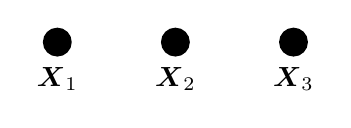
\begin{tikzpicture}[dgraph]
\node[contblk, label=below:{$\boldsymbol X_1$}] (x1) at (1.5, -1.5) {};
\node[contblk, label=below:{$\boldsymbol  X_3$}] (x2) at (4.5,-1.5) {};
\node[contblk, label=below:{$\boldsymbol  X_2$}] (x5) at (3,-1.5) {};
\end{tikzpicture}}
\end{center}	
\caption{Graphical model relating the random variables of the problem with $N=3$.}
 \end{marginfigure}  
For example, if $K=6$ the probability of $x_3=1$ is
\begin{equation*}
  p(\mathbf x = [0,0,1,0,0,0] \mid \boldsymbol \mu) = \mu_1^0 \cdot  \mu_2^0 \cdot \mu_3^1\cdot \mu_4^0\cdot \mu_5^0 \cdot \mu_6^0 = \mu_3
 \end{equation*}
 \item Show that $\sum_{\mathbf x} p(\mathbf x;\boldsymbol \mu) = 1$ and $\mathrm E[\mathbf x\mid  \boldsymbol \mu] =\boldsymbol \mu. $

\item Suppose that we have a data set $\mathcal D = \{\mathbf X_1, \mathbf  X_2,\dots, \mathbf  X_N\}$ of observed values of a categorical random variable $\mathbf  X$. Compute the likelihood and the log-likelihood functions.   

\item The   { likelihood function} is:
 \begin{align*}
 L( \mathbf x_1,\mathbf x_2,\cdots,\mathbf  x_N; \boldsymbol \mu ) 
 &= p(\mathbf x_1,\mathbf x_2,\cdots,\mathbf  x_N;\boldsymbol \mu) \\
 &=  p(\mathbf x_1 ;\boldsymbol \mu) p(\mathbf x_2 ; \boldsymbol \mu) \dots p(\mathbf x_N ; \boldsymbol \mu) \\
  &=  p(\mathbf x_1 ) p(\mathbf x_2 ) \dots p(\mathbf x_N ) \\
  &= \prod_{n=1}^N p(\mathbf x_n) \\
 &= \prod_{n=1}^N\prod_{k=1}^K \mu_k^{x_{nk}} = \prod_{k=1}^K \mu_k^{\sum_{n=1}^N x_{nk}} = \prod_{k=1}^K \mu_k^{m_{k}},
 \end{align*}
 where $m_k = \sum_{n=1}^N x_{nk}$,  and $\sum_{k=1}^K m_k = N$.
 \item The   {log-likelihood function} is:
\begin{align*}
 LL(  \mathbf x_1,\mathbf x_2,\cdots,\mathbf  x_N; \boldsymbol \mu )  &= \log \left[ \prod_{k=1}^K \mu_k^{m_{k}} \right] = \sum_{k=1}^K m_k \log(\mu_k)\\
 &= m_1 \log(\mu_1) + m_2 \log(\mu_2) + m_3 \log(\mu_3) \\
 &+ m_4 \log(\mu_4) + m_5 \log(\mu_5) + m_6 \log(\mu_6)\\
 &= m_1 \log(\mu_1) + m_2 \log(\mu_2) + m_3 \log(\mu_3) \\
 &+ m_4 \log(\mu_4) + m_5 \log(\mu_5) \\ 
 &+   (N-\sum_{n=1}^5 m_n)\log(1-\sum_{n=1}^5 \mu_n)
 \end{align*} 
 \item Show that the maximum likelihood estimate of $\hat \mu_k$ is $\frac{m_k}{N}$, i.e., solve
 $$ \hat{\boldsymbol \mu}_{\text{MLE}} = \arg \max_{\boldsymbol \mu} LL(  \mathbf x_1,\mathbf x_2,\cdots,\mathbf  x_N; \boldsymbol \mu ). $$ 
 To find $\hat{\boldsymbol \mu}_{\text{MLE}} $  we need to solve the following equations system (recall that $\frac{d}{dx}\log x=\frac{1}{x}$):
$$\frac{\partial}{\partial \mu_r}LL(  \mathbf x_1,\mathbf x_2,\cdots,\mathbf  x_N; \boldsymbol \mu ) = \frac{m_r}{\mu_r} - \frac{(N-\sum_{n=1}^5 m_n)}{1-\sum_{n=1}^5 \mu_n}  = 0,$$
where $r=1,2,3,4,5$; $c= N-m_1-m_2-\dots-m_{K-1}$ and
\begin{equation*}
\begin{bmatrix}
(1+\frac{c}{m_1}) & 1 & 1 & \dots & 1\\
1 &  (1+\frac{c}{m_2})  & 1 & \dots & 1\\
1 & 1 & (1+\frac{c}{m_3}) & \dots & 1\\
   &    &  \dots  & & \\ 
1 & 1 & 1 & \dots & (1+\frac{c}{{m_{K-1}}})\\
\end{bmatrix}
\begin{bmatrix}
\mu_1 \\
\mu_2 \\
\mu_3 \\
\dots\\
\mu_{K-1} \\
\end{bmatrix} =
\begin{bmatrix}
1 \\
1 \\
1\\
\dots\\
1 \\
\end{bmatrix}.
\end{equation*}
The solution for this equations system is $\mu_r = \frac{m_r}{N}$, which leds to  $\hat{\boldsymbol \mu}_{\text{MLE}}=(\frac{m_1}{N}, \frac{m_2}{N},\dots,\frac{m_K}{N})$.
 \end{itemize}


\begin{marginfigure}
\begin{center}
\scalebox{0.8}{
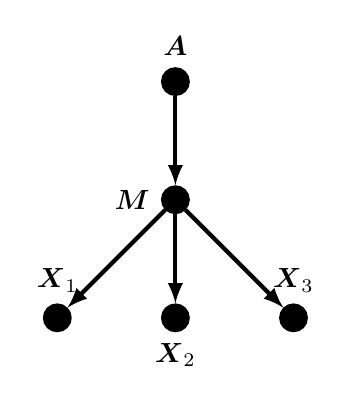
\begin{tikzpicture}[dgraph]
\node[contblk,label=above:{$\boldsymbol A$}] (x3) at (3,1.5) {};
\node[contblk, label=above:{$\boldsymbol X_1$}] (x1) at (1.5, -1.5) {};
\node[contblk, label=left:{$\boldsymbol  M$}] (x4) at (3, -0) {};
\node[contblk, label=above:{$\boldsymbol  X_3$}] (x2) at (4.5,-1.5) {};
\node[contblk, label=below:{$\boldsymbol  X_2$}] (x5) at (3,-1.5) {};
\draw [-{latex[slant=0]}] (x4) -- (x1);
\draw [-{latex[slant=0]}]  (x4) -- (x2);
\draw [-{latex[slant=0]}]  (x4) -- (x5);
\draw [-{latex[slant=0]}]  (x3) -- (x4);
\end{tikzpicture}}
\end{center}	
\caption{Graphical model relating the random variables of the problem with $N=3$.}
 \end{marginfigure}

\subsection{Bayesian Inference}
Bayesian inference is a statistical framework used to update beliefs or make predictions about uncertain events based on prior knowledge and observed evidence. At its core, it involves combining prior beliefs with new evidence to generate a posterior probability distribution, which represents updated beliefs given the data observed. 

The process begins with establishing prior beliefs or probabilities about the parameters of interest. Then, as new data becomes available, Bayes' theorem is applied to update these prior beliefs in light of the observed evidence. The theorem states that the posterior probability is proportional to the product of the prior probability and the likelihood of the data given the parameters. 

In practical terms, Bayesian inference allows for a flexible approach to modeling uncertainty, incorporating both subjective prior beliefs and objective data. It's widely used in various fields such as machine learning, medical diagnosis, and decision-making, offering a coherent framework for reasoning under uncertainty. However, it requires careful specification of prior beliefs and can be computationally intensive, particularly for complex models.

\subsection{Example 2}

Let  $ \{\mathbf X_1,\mathbf X_2,\dots, \mathbf X_N\}$ be a set of i.d.d samples of a categorical variable  $\mathbf X \sim \mathsf{Categorical}(\mathbf x\mid \boldsymbol \mu)$. 
\begin{align*}
p(\mathbf x_1,\mathbf x_2,\dots, \mathbf x_N,  \boldsymbol \mu, \boldsymbol \alpha  ) &=  p(\boldsymbol \mu\mid \boldsymbol \alpha)p(\boldsymbol \alpha)  \prod_{n=1}^N p(\mathbf x_n \mid \boldsymbol \mu)\\
&=  p(\boldsymbol \mu,\boldsymbol \alpha) \underbrace{\prod_{n=1}^N p(\mathbf x_n \mid \boldsymbol \mu)}_{\mathsf{likelihood} }\\
\end{align*}
\begin{itemize}
\item What is the likelihood function of the data?
\begin{align*}
 L(\mathbf x_1,\mathbf x_2,\cdots,\mathbf  x_N\mid \boldsymbol \mu   ) 
  &=  p(\mathbf x_1,\mathbf x_2,\cdots,\mathbf  x_N\mid \boldsymbol \mu) \\
  &= p(\mathbf x_1 \mid \boldsymbol \mu) p(\mathbf x_2 \mid \boldsymbol \mu) \dots p(\mathbf x_N \mid \boldsymbol \mu) \\
  &= \prod_{n=1}^N p(\mathbf x_n \mid \boldsymbol \mu) \\
  & = \prod_{k=1}^K \mu_k^{m_{k}},\\
 LL( \mathbf x_1,\mathbf x_2,\cdots,\mathbf  x_N \mid  \boldsymbol \mu )  &= \log \left[ \prod_{k=1}^K \mu_k^{m_{k}} \right] = \sum_{k=1}^K m_k \log(\mu_k),\\
 \end{align*}
 where $m_k = \sum_{n=1}^N x_{nk}$,  and $\sum_{k=1}^K m_k = N$.
 \begin{marginfigure}
\includegraphics{fig/dirichlet2.pdf}
\caption{Dirichlet distributions over three variables $\mu_1$,$\mu_2$, and $\mu_3$. The distributions are confined to simple as a consequence of the constraints on $\mu_k$. From left to right, Dirichlet distributions for $\{\alpha_k\}=0.1$, $\{\alpha_k\}=1$ and $\{\alpha_k\}= 10$.}
\end{marginfigure}
 
 \item Assume that $\boldsymbol M = (M_1,\dots,M_k)$ has a symmetric Dirichlet distribution with parameter $\boldsymbol \alpha$:
 \begin{align*}
\mathsf{Dirichlet}(\boldsymbol \mu \mid \boldsymbol \alpha) &= \frac{\Gamma(\sum_{k=1}^K\alpha_k)}{\Gamma(\alpha_1)\Gamma(\alpha_2)\cdots\Gamma(\alpha_K)}\prod_{k=1}^K\mu{_k}^{\alpha_k-1},
\end{align*}  
where $0 \leq \mu_k \leq 1$, $\sum_{k=1}^K \mu_k = 1$, $\boldsymbol \alpha = (\alpha_1,\dots,\alpha_k)$ and $\boldsymbol \mu = (\mu_1,\dots,\mu_k)$.\item Compute the posterior distribution $p(\boldsymbol \mu \mid \mathbf x_1,\mathbf x_2,\cdots,\mathbf  x_N, \boldsymbol \alpha)$.
\begin{align*}
p(\boldsymbol \mu \mid \mathbf x_1,\mathbf x_2,\cdots,\mathbf  x_N, \boldsymbol \alpha) &= \frac{p( \mathbf x_1,\mathbf x_2,\cdots,\mathbf  x_N, \boldsymbol \mu, \boldsymbol \alpha)}{p(\mathbf x_1,\mathbf x_2,\cdots,\mathbf  x_N,\boldsymbol   \alpha)}\\
&=\frac{p( \mathbf x_1,\mathbf x_2,\cdots,\mathbf  x_N \mid \boldsymbol \mu,\boldsymbol   \alpha)p(\boldsymbol \mu, \boldsymbol \alpha)}{p(\mathbf x_1,\mathbf x_2,\cdots,\mathbf  x_N,\boldsymbol   \alpha)}\\
&= \frac{p( \mathbf x_1,\mathbf x_2,\cdots,\mathbf  x_N \mid \boldsymbol \mu, \boldsymbol \alpha)p(\boldsymbol \mu\mid \boldsymbol \alpha)p( \boldsymbol \alpha)}{p(\mathbf x_1,\mathbf x_2,\cdots,\mathbf  x_N\mid \boldsymbol  \alpha)p(\boldsymbol  \alpha)}\\
&= \frac{p( \mathbf x_1,\mathbf x_2,\cdots,\mathbf  x_N \mid \boldsymbol \mu)p(\boldsymbol \mu\mid \boldsymbol \alpha)}{p(\mathbf x_1,\mathbf x_2,\cdots,\mathbf  x_N\mid \boldsymbol  \alpha)}\\
&\propto p( \mathbf x_1,\mathbf x_2,\cdots,\mathbf  x_N \mid \boldsymbol \mu)p(\boldsymbol \mu\mid \boldsymbol  \alpha).\\
\end{align*} 
 
This is how we compute the posterior distribution:
\begin{align*}
\underbrace{p( \boldsymbol \mu \mid  \mathbf x_1,\mathbf x_2,\cdots,\mathbf  x_N, \alpha)}_{\mathsf{posterior}}  &\propto \underbrace{p(\mathbf x_1,\mathbf x_2,\cdots,\mathbf  x_N\mid \boldsymbol \mu) }_{\mathsf{likelihood}} \underbrace{p(\boldsymbol \mu\mid \boldsymbol  \alpha)}_{\mathsf{prior}}.
\end{align*}
Therefore we have:
\begin{align*}
p(\mathbf x_1,\mathbf x_2,\cdots,\mathbf  x_N\mid \boldsymbol \mu) \cdot p(\boldsymbol \mu\mid \alpha) &=\prod_{n=1}^N\prod_{k=1}^K \mu_k^{x_{nk}} \cdot
 \frac{\Gamma(K\alpha)}{\Gamma(\alpha)^K} \prod_{k=1}^K \mu{_k}^{\alpha-1}\\
&\propto \prod_{k=1}^K \mu_k^{\sum_{n=1}^Nx_{nk} + \alpha - 1} \\
&\propto  \frac{\Gamma(\sum_{k=1}^K (x_{\cdot k} + \alpha))}{\Gamma(x_{\cdot 1} + \alpha)\cdots\Gamma(x_{\cdot K} + \alpha)} \prod_{k=1}^K \mu_k^{x_{\cdot k} + \alpha - 1}\\
&= \mathsf{Dirichlet}(\boldsymbol \mu \mid \boldsymbol  \alpha')\\
&= p(\boldsymbol \mu \mid \mathbf x_1,\mathbf x_2,\cdots,\mathbf  x_N,  \alpha),
\end{align*}
with $x_{\cdot k} = \sum_{n=1}^Nx_{nk}$, and $\boldsymbol \alpha' = (x_{\cdot 1} + \alpha,\dots,x_{\cdot  K} + \alpha)$. Notice that the expected value of $\alpha_k'$ is 
\begin{equation*}
E_{\boldsymbol \mu \mid \mathbf x_1,\mathbf x_2,\cdots,\mathbf  x_N,  \alpha}[\mu_k] =  E[\mu_k\mid \mathbf x_1,\mathbf x_2,\cdots,\mathbf  x_N,  \alpha]= \frac{x_{\cdot  k} + \alpha}{ \sum_{k=1}^K(x_{\cdot  k} + \alpha)} = \frac{x_{\cdot  k} + \alpha}{x_{\cdot  \cdot} + K\alpha}.
\end{equation*}
\end{itemize}

\subsection{Example 3}

Let  $ \{ X_1, X_2,\dots,  X_L\}$ be a data set of observed values of a Binomial random variable 
\begin{align*}
p(x\mid\mu) = {N\choose x}\mu^x(1-\mu)^{(1-x)}
\end{align*}

\begin{align*}
p( x_1, x_2,\dots,  x_L,  \mu, \alpha, \beta  ) &=  p(\mu\mid \alpha,\beta)p( \alpha)p(\beta)  \prod_{n=1}^L p( x_n \mid \mu)\\
&=  p( \mu, \alpha, \beta) \underbrace{\prod_{n=1}^L p(\mathbf x_n \mid \boldsymbol \mu)}_{\mathsf{likelihood} }\\
\end{align*}


  Compute the posterior distribution and the expected value of a  Beta prior. (Hint $n=\sum_{l=1}^L x_l).$ 
 \begin{marginfigure}
\begin{center}
\scalebox{0.8}{
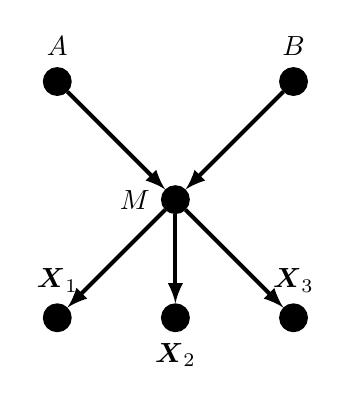
\begin{tikzpicture}[dgraph]
\node[contblk,label=above:{$A$}] (x3) at (1.5,1.5) {};
\node[contblk,label=above:{$B$}] (x6) at (4.5,1.5) {};
\node[contblk, label=above:{$\boldsymbol X_1$}] (x1) at (1.5, -1.5) {};
\node[contblk, label=left:{$M$}] (x4) at (3, -0) {};
\node[contblk, label=above:{$\boldsymbol  X_3$}] (x2) at (4.5,-1.5) {};
\node[contblk, label=below:{$\boldsymbol  X_2$}] (x5) at (3,-1.5) {};
\draw [-{latex[slant=0]}] (x4) -- (x1);
\draw [-{latex[slant=0]}]  (x4) -- (x2);
\draw [-{latex[slant=0]}]  (x4) -- (x5);
\draw [-{latex[slant=0]}]  (x3) -- (x4);
\draw [-{latex[slant=0]}]  (x6) -- (x4);
\end{tikzpicture}}
\end{center}	
\caption{Graphical model relating the binomial random variables of the problem with $L=3$.}
 \end{marginfigure}
  
  
  
 \begin{itemize}
 \item The prior distribution is given by 
 \begin{align*}
 p(\mu\mid\alpha,\beta)  = \mathsf{Beta}(\mu\mid \alpha, \beta) = \frac{\Gamma(\alpha+\beta)}{\Gamma(\alpha)\Gamma(\beta)}x^{\alpha-1}(1-x)^{\beta-1}.
 \end{align*}
 \item  The likelihood of the data is given by 
  \begin{align*}
p( x_1,  x_2,\dots,  x_L\mid \mu) &= \prod_{l=1}^L p(x_l\mid {\mu}) =  \prod_{l=1}^L \mathsf{Binomial}(x_l\mid \mu) \\
&=  \prod_{l=1}^L  {{N}\choose x_l} {\mu}^{x_l} {(1-\mu)}^{{N}-x_l}  \\
&= \left[\prod_{l=1}^L  {{N}\choose x_l} \right] {\mu}^{n}{(1-\mu)}^{{LN}-n}.  \\
%p(\mu \mid x_1,x_2,\dots,x_L)&\propto \mathsf{\mu}^{n}\mathsf{(1-\mu)}^{{LN}-n}.
\end{align*}
\item The posterior distribution is proportional to the likelihood and the prior.
 \begin{align*}
\underbrace{p(\mu\mid x_1,\dots,x_L,\alpha,\beta)}_{\mathsf{posterior}}  &\propto \underbrace{ \prod_{l=1}^L p(x_l\mid{\mu})}_{{likelihood}} \underbrace{p(\mu\mid\alpha,\beta)}_{{prior}}.
\end{align*}


\item The posterior distribution is
 \begin{align*}
p(\mu \mid x_1,x_2,\dots,x_L,\alpha,\beta) &\propto {\mu}^{n+\alpha-1}{(1-\mu)}^{{LN}-n+\beta-1}\\
&=  \mathsf{Beta}(\mu\mid n + \alpha,LN-n+\beta).
\end{align*}
 \item The posterior distribution is proportional to the likelihood and the prior.
  \begin{marginfigure}
\begin{center}
  \begin{tabular}{ rrrrcc}
    \hline
    $\alpha$ & $\beta$ & $L$ & $N$ & $\mathrm E[M]$ & $\mathrm{Var}[M]$  \\\hline\hline
    1 & 1 & 10 & 1 & 0.67 & 0.0170\\ 
    1 & 1 & 100 &1 & 0.64 & 0.0220\\
    1 & 1 & 1000 &1 & 0.49 & 0.0002\\
    1 & 1 & 10000& 1& 0.49& 2.499e-5\\
    1 & 1 &100 &100 &0.50 &2.499e-5\\
    2 & 2 &10 &1&  0.43 &0.0160  \\ 
    40 & 40 & 10 &  1& 0.51 & 0.0027\\
    400 & 400 & 10 &  1& 0.50 & 0.0003\\    
     \hline
  \end{tabular}
    \small Data were generated with $\mu=0.5$.
\end{center}
 \end{marginfigure}
 \begin{align*}
\underbrace{p(\mu\mid x_1,\dots,x_L,\alpha,\beta)}_{\mathsf{posterior}}  &\propto \underbrace{ \prod_{l=1}^L p(x_l\mid{\mu})}_{{likelihood}} \underbrace{p(\mu\mid\alpha,\beta)}_{{prior}}.
\end{align*}
\item The posterior distribution is
 \begin{align*}
p(\mu \mid x_1,x_2,\dots,x_L,\alpha,\beta) &\propto{\mu}^{n+\alpha-1}{(1-\mu)}^{{LN}-n+\beta-1}\\
&=  \mathsf{Beta}(\mu\mid n + \alpha,LN-n+\beta).
\end{align*}
\item Notice that the posterior expected value and variance of $M$ are:
 \begin{align*}
\mathrm E[M] = \frac{n+ \alpha}{LN+\alpha+\beta}.
\end{align*}
 \begin{align*}
\mathrm{var}[M] = \frac{(n+ \alpha)(LN-n+\beta)}{(LN+\alpha+\beta)^2(LN+\alpha+\beta + 1)}.
\end{align*}
\end{itemize}

\begin{figure}
\includegraphics[width=8cm]{fig/posterior_panel.pdf}
\caption{From top to bottom: $L=10,N=1$; $L=100,N=1$; $L=1000,N=1$; $L=100,N=100$;  $L=10,N=1$. Bottom row: non-uniform  prior $\alpha=2$, and $\beta=2$.}
\end{figure}

\begin{mybox}{Example: Bernoulli Distribution}{theoexample}
\begin{itemize}
 \item The evaluation of drugs for possible clinical application, studies are routinely performed on
 rodents. For a particular study, suppose that the immediate aim is to estimate $M$, the
 probability of Parkinson's in a population of female laboratory rats that receive a small dose
 of a drug to prevent the disease. The population of rodents consists of   50  groups. Each group consists of 10 individuals.
 \item Use the data shown below to compute the posterior probability of Parkinson's in the population, assuming a uniform beta
 prior.
 \item  The number of healthy individuals after the application of the drug for each group are {\sf 5, 4, 7, 5, 4, 5, 6, 4, 6, 7, 6, 6, 9, 7, 2, 4, 9, 5, 8, 8, 6, 7, 7, 7, 4,  8, 5, 5, 2, 5, 4, 7, 5, 5, 4, 8, 6, 7, 5, 6, 5, 6, 6, 8, 4, 7, 8, 3, 7, 6,} respectively.
 \end{itemize}
\end{mybox}
\begin{figure}
\includegraphics[width=9cm]{fig/birth.pdf}
\caption{Posterior inference model.}
\end{figure}

\subsection{Annex 1}

We thank Julio Cesar Mart\'{i}nez S\'{a}nchez for developing the calculations of Example 1.

Verificar
 
\begin{eqnarray}
\hat{\mu} = \frac{\partial}{\partial \mu_r} \ell(\mu; x_1, x_2, x_3, x_4, x_5) = \frac{m_r}{\mu_r} - \frac{N - \sum_{n=1}^{5} m_n}{1- \sum_{n=1}^{5} \mu_n} 
\end{eqnarray}

sea $c= N - \sum_{n=1}^{5} m_n$, la derivada parcial con respecto a $\mu_1$ viene dada por 

\begin{eqnarray*}
\frac{\partial}{\partial \mu_1} \ell(\mu; x_1, x_2, x_3, x_4, x_5) = \frac{m_1}{\mu_1} - \frac{c}{1- \sum_{n=1}^{5} \mu_n}
\end{eqnarray*}

igualando a cero 

\begin{eqnarray*}
\frac{m_1}{\mu_1} - \frac{c}{1- \sum_{n=1}^{5} \mu_n} = 0
\end{eqnarray*}

resolviendo la fracción

\begin{eqnarray*}
\frac{m_1(1- \sum_{n=1}^{5} \mu_n)  - \mu_1 c}{\mu_1 (1- \sum_{n=1}^{5} \mu_n)} & = & 0 \\
m_1(1- \sum_{n=1}^{5} \mu_n)  - \mu_1 c & = & 0\\
m_1 - m_1 \sum_{n=1}^{5} \mu_n - \mu_1 c & = & 0\\
m_1 - m_1(\mu_1 + \mu_2 + \mu_3 + \mu_4 + \mu_5) - \mu_1 c & = & 0\\
\end{eqnarray*}

dividimos entre $m_1$, y simplificando
\begin{eqnarray*}
\frac{m_1}{m_1} - \frac{m_1}{m_1}(\mu_1 + \mu_2 + \mu_3 + \mu_4 + \mu_5) - \frac{\mu_1}{m_1} c & = & 0\\
1 - (\mu_1 + \mu_2 + \mu_3 + \mu_4 + \mu_5) - \frac{\mu_1}{m_1} c & = & 0\\
1 - \mu_1 - \mu_2 - \mu_3 - \mu_4 - \mu_5 - \frac{\mu_1}{m_1} c & = & 0\\
\end{eqnarray*}

agrupando los términos con $\mu_1$
\begin{eqnarray*}
1 - \mu_1 - \frac{\mu_1}{m_1}c  -\mu_2 - \mu_3 - \mu_4 - \mu_5 & = & 0 \\
1 - \mu_1\left(1 + \frac{c}{m_1}\right)  -\mu_2 - \mu_3 - \mu_4 - \mu_5 & = & 0 \\
\end{eqnarray*}
despejando el $1$
\begin{eqnarray*}
 \mu_1\left(1 + \frac{c}{m_1}\right)  + \mu_2 + \mu_3 + \mu_4 + \mu_5  & = & 1\\
\end{eqnarray*}

note que para la derivada parcial con respecto a $\mu_2$ es el mismo procedimiento, es decir,

\begin{eqnarray*}
 \mu_1 + \mu_2\left(1 + \frac{c}{m_2}\right)  + \mu_3 + \mu_4 + \mu_5  & = & 1\\
\end{eqnarray*}

la derivada parcial con respecto a $\mu_3$

\begin{eqnarray*}
 \mu_1 + \mu_2 + \mu_3\left(1 + \frac{c}{m_3}\right)  +  \mu_4 + \mu_5  & = & 1\\
\end{eqnarray*}

en resumen, vamos a tener para todas las derivadas parciales el siguiente sistema de ecuaciones

\begin{eqnarray*}
\mu_1\left(1 + \frac{c}{m_1}\right)  +\mu_2 + \mu_3 + \mu_4 + \mu_5 & = & 1 \\
 \mu_1 + \mu_2\left(1 + \frac{c}{m_2}\right)  + \mu_3 + \mu_4 + \mu_5  & = & 1\\
  \mu_1 + \mu_2 + \mu_3\left(1 + \frac{c}{m_3}\right)  +  \mu_4 + \mu_5  & = & 1\\
  \mu_1 + \mu_2 + \mu_3  + \mu_4\left(1 + \frac{c}{m_4}\right)  + \mu_5  & = & 1\\
    \mu_1 + \mu_2 + \mu_3  + \mu_4 + \mu_5\left(1 + \frac{c}{m_5}\right) & = & 1\\
\end{eqnarray*}

en términos matriciales

\begin{equation}
\begin{bmatrix}
   \left(1 + \frac{c}{m_1}\right) & 1 & 1 & 1 & 1 \\
	1 & \left(1 + \frac{c}{m_2}\right) & 1 & 1 & 1 \\
	1 & 1 & \left(1 + \frac{c}{m_3}\right) & 1 & 1  \\
	1 & 1 & 1 & \left(1 + \frac{c}{m_4}\right) & 1  \\
	1 & 1 & 1 & 1 &\left(1 + \frac{c}{m_5}\right)  \\
\end{bmatrix}
\begin{bmatrix}
   \mu_1 \\
   \mu_2 \\
	\mu_3 \\
	\mu_4 \\
	\mu_5 \\
\end{bmatrix}
=
\begin{bmatrix}
   1 \\
   1 \\
   1 \\
   1\\
   1\\
\end{bmatrix}
\end{equation}


 \begin{figure}
\begin{center}
\scalebox{0.8}{
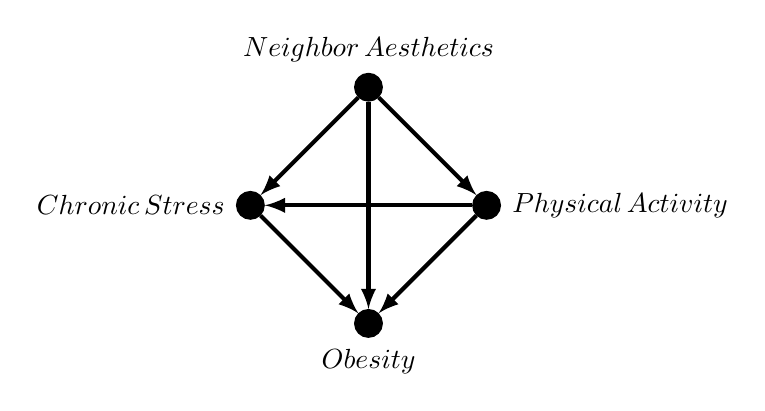
\begin{tikzpicture}[dgraph]
\node[contblk, label=above:{$Neighbor\,Aesthetics$}] (NA) at (3, 3) {};
\node[contblk,label=left:{$Chronic\,  Stress$}] (CS) at (1.5,1.5) {};
\node[contblk,label=right:{$Physical\, Activity$}] (PA) at (4.5,1.5) {};
\node[contblk, label=below:{$Obesity$}] (OB) at (3, -0) {};
\draw [-{latex[slant=0]}] (NA) -- (CS);
\draw [-{latex[slant=0]}] (NA) -- (PA);
\draw [-{latex[slant=0]}] (CS) -- (OB);
\draw [-{latex[slant=0]}] (PA) -- (OB);
\draw [-{latex[slant=0]}] (NA) -- (OB);
\draw [-{latex[slant=0]}] (PA) -- (CS);
\end{tikzpicture}}
\end{center}	
\caption{Graphical model relating the binomial random variables of the problem with $L=3$.}
 \end{figure}


%\end{mybox}

\vspace{1cm}

\vspace{1cm}
\end{document}


